\documentclass[C++.tex]{subfiles}
\begin{document}

\section{C++17}
\subsection*{Présentation}
\begin{frame}
	\frametitle{Présentation}
	\begin{itemize}
		\item Approuvé en décembre 2017
		\item Dernier Working Draft : \href{http://www.open-std.org/jtc1/sc22/wg21/docs/papers/2017/n4659.pdf}{N4659}
		\item Support complet du langage par Clang, GCC et Visual C++
		\item Très bon support de la bibliothèque par Clang, GCC et Visual C++
		\item Progression très rapide du support en parallèle de la normalisation
	\end{itemize}

	\begin{block}{Note}
		\begin{itemize}
			\item Voir \href{https://www.youtube.com/user/lefticus1/videos}{Vidéos C++ Weekly} (Jason Turner)
		\end{itemize}
	\end{block}
\end{frame}

\subsection*{Suppression}
\begin{frame}[fragile]
	\frametitle{Fonctionnalités supprimées}
	\begin{itemize}
		\item Suppression des trigraphes (non dépréciés)
	\end{itemize}

	\begin{block}{Note}
		\begin{itemize}
			\item Les digraphes ne sont pas concernés
		\end{itemize}
	\end{block}

	\begin{itemize}
		\item Suppression de \lstinline|register| (qui reste un mot réservé)
		\item Suppression des opérateurs d'incrément sur les booléens

\note[item]{\lstinline|operator++| déjà déprécié en C++98}

		\item Suppression de \lstinline|std::auto_ptr|
		\item Suppression de \lstinline|std::random_shuffle()|
		\item Suppression des anciens mécanismes fonctionnels : \lstinline|std::bind1st()|, \lstinline|std::bind2nd()|, \ldots
		\item Suppression des spécifications d'exception
	\end{itemize}
\end{frame}

\subsection*{include}
\begin{frame}[fragile]
	\frametitle{\lstinline|__has_include|}
	\begin{itemize}
		\item Teste la présence d'un fichier d'en-tête
		\item Et donc la disponibilité d'une fonctionnalité
	\end{itemize}

	\begin{lstlisting}[language=C++]
#if __has_include(<optional>)
#  include <optional>
#  define OPT_ENABLE
#endif\end{lstlisting}

	\vskip 10mm plus 10fill
	\hfill
	\href{https://godbolt.org/#g:!((g:!((g:!((h:codeEditor,i:(filename:'1',fontScale:14,fontUsePx:'0',j:1,lang:c%2B%2B,selection:(endColumn:1,endLineNumber:11,positionColumn:1,positionLineNumber:11,selectionStartColumn:1,selectionStartLineNumber:1,startColumn:1,startLineNumber:1),source:'%23include+%3Ciostream%3E%0A%23if+__has_include(%3Coptional%3E)%0A%23++include+%3Coptional%3E%0A%23++define+OPT_ENABLE+1%0A%23endif%0A%0Aint+main()%0A%7B%0A++std::cout+%3C%3C+OPT_ENABLE+%3C%3C+%22%5Cn%22%3B%0A%7D%0A'),l:'5',n:'0',o:'C%2B%2B+source+%231',t:'0')),k:50,l:'4',n:'0',o:'',s:0,t:'0'),(g:!((h:executor,i:(argsPanelShown:'1',compilationPanelShown:'0',compiler:g122,compilerName:'',compilerOutShown:'0',execArgs:'',execStdin:'',fontScale:14,fontUsePx:'0',j:1,lang:c%2B%2B,libs:!((name:boost,ver:'175')),options:'-std%3Dc%2B%2B17+-Wall+-Wextra',source:1,stdinPanelShown:'1',tree:'1',wrap:'0'),l:'5',n:'0',o:'Executor+x86-64+gcc+12.2+(C%2B%2B,+Editor+%231)',t:'0')),header:(),k:50,l:'4',n:'0',o:'',s:0,t:'0')),l:'2',n:'0',o:'',t:'0')),version:4}{
\includegraphics[height=0.5cm]{input_src/play-button.png}}
\end{frame}

\subsection*{inline variable}
\begin{frame}[fragile]
	\frametitle{inline variable}
	\begin{itemize}
		\item Sémantique \lstinline|inline| identique sur fonctions et variables
		\item Peut être définie, à l'identique, dans plusieurs unité de compilation
		\item Se comporte comme s'il n'y avait qu'une variable
	\end{itemize}

	\begin{lstlisting}[language=C++]
inline int foo = 42;\end{lstlisting}

	\begin{itemize}
		\item \lstinline|constexpr| sur une donnée membre statique implique \lstinline|inline|
		\item Utile pour initialiser des variables membres statiques non constantes
	\end{itemize}

	\begin{lstlisting}[language=C++]
class Foo { static inline int bar = 42; };\end{lstlisting}

	\begin{alertblock}{Don't}
		\begin{itemize}
			\item Ne justifie pas l'usage de variables globales
		\end{itemize}
	\end{alertblock}
\end{frame}

\subsection*{Namespace}
\begin{frame}[fragile]
	\frametitle{Nested namespace}
	\begin{itemize}
		\item Simplification des imbrications de namespaces via l'opérateur \lstinline|::| 
	\end{itemize}

	\begin{lstlisting}[language=C++]
namespace A {
namespace B {
namespace C {
...
}}}

// Devient

namespace A::B::C {
...
}\end{lstlisting}

	\vskip 10mm plus 10fill
	\hfill
	\href{https://godbolt.org/#g:!((g:!((g:!((h:codeEditor,i:(filename:'1',fontScale:14,fontUsePx:'0',j:1,lang:c%2B%2B,selection:(endColumn:1,endLineNumber:12,positionColumn:1,positionLineNumber:12,selectionStartColumn:1,selectionStartLineNumber:1,startColumn:1,startLineNumber:1),source:'%23include+%3Ciostream%3E%0A%0Anamespace+A::B::C%0A%7B%0A++int+foo+%3D+5%3B%0A%7D%0A%0Aint+main()%0A%7B%0A++std::cout+%3C%3C+A::B::C::foo+%3C%3C+%22%5Cn%22%3B%0A%7D%0A'),l:'5',n:'0',o:'C%2B%2B+source+%231',t:'0')),k:50,l:'4',n:'0',o:'',s:0,t:'0'),(g:!((h:executor,i:(argsPanelShown:'1',compilationPanelShown:'0',compiler:g122,compilerName:'',compilerOutShown:'0',execArgs:'',execStdin:'',fontScale:14,fontUsePx:'0',j:1,lang:c%2B%2B,libs:!((name:boost,ver:'175')),options:'-std%3Dc%2B%2B17+-Wall+-Wextra+-pedantic',source:1,stdinPanelShown:'1',tree:'1',wrap:'0'),l:'5',n:'0',o:'Executor+x86-64+gcc+12.2+(C%2B%2B,+Editor+%231)',t:'0')),header:(),k:50,l:'4',n:'0',o:'',s:0,t:'0')),l:'2',n:'0',o:'',t:'0')),version:4}{
\includegraphics[height=0.5cm]{input_src/play-button.png}}
\end{frame}

\subsection*{static\_assert}
\begin{frame}[fragile]
	\frametitle{\lstinline|static_assert| sans message}
	\begin{itemize}
		\item \lstinline|static_assert| sans message utilisateur
	\end{itemize}

	\begin{lstlisting}[language=C++]
static_assert(sizeof(int) == 3);
// Erreur de compilation\end{lstlisting}

	\vskip 10mm plus 10fill
	\hfill
	\href{https://godbolt.org/#g:!((g:!((g:!((h:codeEditor,i:(filename:'1',fontScale:14,fontUsePx:'0',j:1,lang:c%2B%2B,selection:(endColumn:1,endLineNumber:7,positionColumn:1,positionLineNumber:7,selectionStartColumn:1,selectionStartLineNumber:1,startColumn:1,startLineNumber:1),source:'%23include+%3Ciostream%3E%0A%0Aint+main()%0A%7B%0A++static_assert(sizeof(int)+%3D%3D+3)%3B%0A%7D%0A'),l:'5',n:'0',o:'C%2B%2B+source+%231',t:'0')),k:50,l:'4',n:'0',o:'',s:0,t:'0'),(g:!((h:executor,i:(argsPanelShown:'1',compilationPanelShown:'0',compiler:g122,compilerName:'',compilerOutShown:'0',execArgs:'',execStdin:'',fontScale:14,fontUsePx:'0',j:1,lang:c%2B%2B,libs:!((name:boost,ver:'175')),options:'-std%3Dc%2B%2B17+-Wall+-Wextra+-pedantic',source:1,stdinPanelShown:'1',tree:'1',wrap:'0'),l:'5',n:'0',o:'Executor+x86-64+gcc+12.2+(C%2B%2B,+Editor+%231)',t:'0')),header:(),k:50,l:'4',n:'0',o:'',s:0,t:'0')),l:'2',n:'0',o:'',t:'0')),version:4}{
\includegraphics[height=0.5cm]{input_src/play-button.png}}
\end{frame}

\subsection*{if constexpr}
\begin{frame}[fragile]
	\frametitle{\lstinline|if constexpr|}
	\begin{itemize}
		\item Branchement évalué à la compilation
	\end{itemize}

	\begin{lstlisting}[language=C++]
if constexpr(cond) {
  ... }
else if constexpr(cond) {
  ... }
else {
  ... }\end{lstlisting}

	\begin{itemize}
		\item Conditions d'arrêt plus simple avec les \textit{variadic template}
		\item Moins de spécialisations explicites
	\end{itemize}

	\begin{block}{Note}
		\begin{itemize}
			\item Conditions intégralement évaluables au \textit{compile-time}, pas de court-circuit
		\end{itemize}

\note[item]{C'est à dire qu'en cas de condition composée (\lstinline|or|, \lstinline|and|), même si la première partie permet de résoudre la condition, il faut que le reste soit évaluable en \textit{compile-time}}
	\end{block}
\end{frame}

\begin{frame}[fragile]
	\frametitle{\lstinline|if constexpr|}
	\begin{lstlisting}[language=C++]
template <typename T> auto foo(T t) {
if constexpr(is_pointer_v<T>)
  return *t;
else
  return t;}

int a = 10, b = 5;
int* ptr = &b;
cout << foo(a) << ' ' << foo(ptr);  // 10 5\end{lstlisting}
\end{frame}

\begin{frame}[fragile]
	\frametitle{\lstinline|if constexpr|}
	\begin{block}{Note}
		\begin{itemize}
			\item Les branches doivent être syntaxiquement correctes mais pas nécessairement sémantiquement valides
		\end{itemize}
	\end{block}

	\begin{block}{Note}
		\begin{itemize}
			\item Les branches peuvent avoir des types retour différents sans remettre en cause la déduction de type retour
		\end{itemize}
	\end{block}

	\begin{exampleblock}{Do}
		\begin{itemize}
			\item Préférez \lstinline|if constexpr| aux suites de spécialisations de template et SFINAE, aux imbrications de ternaires ou à \lstinline|#if|
		\end{itemize}
	\end{exampleblock}
\end{frame}

\begin{frame}[fragile]
	\frametitle{\lstinline|if constexpr|}
	\begin{block}{\textit{hello world} de la récursion}
		\begin{lstlisting}[language=C++]
template<int  N>
constexpr int fibo(){ return fibo<N-1>()+fibo<N-2>(); }
template<>
constexpr int fibo<1>() { return 1; }
template<>
constexpr int fibo<0>() { return 0; }

// Devient

template<int N>
constexpr int fibo() {
  if constexpr (N>=2) return fibo<N-1>()+fibo<N-2>();
  else return N; }\end{lstlisting}
	\end{block}

	\hfill
	\href{https://godbolt.org/#g:!((g:!((g:!((h:codeEditor,i:(filename:'1',fontScale:14,fontUsePx:'0',j:1,lang:c%2B%2B,selection:(endColumn:1,endLineNumber:31,positionColumn:1,positionLineNumber:31,selectionStartColumn:1,selectionStartLineNumber:1,startColumn:1,startLineNumber:1),source:'%23include+%3Ciostream%3E%0A%0Atemplate+%3Ctypename+T%3E+auto+foo(T+t)%0A%7B%0A++if+constexpr+(std::is_pointer_v%3CT%3E)%0A++++return+*t%3B%0A++else%0A++++return+t%3B%0A%7D%0A%0Atemplate%3Cint+N%3E%0Aconstexpr+int+fibo()%0A%7B%0A++if+constexpr+(N%3E%3D2)%0A++++return+fibo%3CN-1%3E()%2Bfibo%3CN-2%3E()%3B%0A++else+return+N%3B%0A%7D%0A%0Aint+main()%0A%7B%0A++%7B%0A++++int+a+%3D+10,+b+%3D+5%3B%0A++++int*+ptr+%3D+%26b%3B%0A++++std::cout+%3C%3C+foo(a)+%3C%3C+!'+!'+%3C%3C+foo(ptr)+%3C%3C+!'%5Cn!'%3B%0A++%7D%0A%0A++%7B%0A++++std::cout+%3C%3C+fibo%3C8%3E()+%3C%3C+!'%5Cn!'%3B%0A++%7D%0A%7D%0A'),l:'5',n:'0',o:'C%2B%2B+source+%231',t:'0')),k:50,l:'4',n:'0',o:'',s:0,t:'0'),(g:!((h:executor,i:(argsPanelShown:'1',compilationPanelShown:'0',compiler:g122,compilerName:'',compilerOutShown:'0',execArgs:'',execStdin:'',fontScale:14,fontUsePx:'0',j:1,lang:c%2B%2B,libs:!((name:boost,ver:'175')),options:'-std%3Dc%2B%2B17+-Wall+-Wextra+-pedantic',source:1,stdinPanelShown:'1',tree:'1',wrap:'0'),l:'5',n:'0',o:'Executor+x86-64+gcc+12.2+(C%2B%2B,+Editor+%231)',t:'0')),header:(),k:50,l:'4',n:'0',o:'',s:0,t:'0')),l:'2',n:'0',o:'',t:'0')),version:4}{
\includegraphics[height=0.5cm]{input_src/play-button.png}}
\end{frame}

\subsection*{init statement}
\begin{frame}[fragile]
	\frametitle{if init statement}
	\begin{itemize}
		\item Initialisation dans le branchement
		\item Portée identique aux déclarations dans la condition
	\end{itemize}

	\begin{lstlisting}[language=C++]
if(int foo = 42; bar)   cout << foo;
else                    cout << -foo;\end{lstlisting}

	\begin{itemize}
		\item Sémantiquement équivalent à
	\end{itemize}

	\begin{lstlisting}[language=C++]
{
  int foo = 42;
  if(bar)  cout << foo;
  else     cout << -foo;
}\end{lstlisting}
\end{frame}

\begin{frame}[fragile]
	\frametitle{if init statement}
	\begin{itemize}
		\item Alternative à certaines constructions peu lisibles
	\end{itemize}

	\begin{lstlisting}[language=C++]
if((bool ret = foo()) == true) ...\end{lstlisting}

	\begin{itemize}
		\item \ldots{} injectant un symbole inutile au delà du branchement
	\end{itemize}

	\begin{lstlisting}[language=C++]
bool ret = foo();
if(ret) ...\end{lstlisting}

	\begin{itemize}
		\item \ldots{} nécessitant l'introduction d'une portée supplémentaire
	\end{itemize}

	\begin{lstlisting}[language=C++]
{
  bool ret = foo();
  if(ret) ...
}\end{lstlisting}

	\hfill
	\href{https://godbolt.org/#g:!((g:!((g:!((h:codeEditor,i:(filename:'1',fontScale:14,fontUsePx:'0',j:1,lang:c%2B%2B,selection:(endColumn:1,endLineNumber:16,positionColumn:1,positionLineNumber:16,selectionStartColumn:1,selectionStartLineNumber:1,startColumn:1,startLineNumber:1),source:'%23include+%3Ciostream%3E%0A%0Aint+main()%0A%7B%0A++int+bar+%3D+5%3B%0A%0A++if(int+foo+%3D+42%3B+bar)%0A++%7B%0A++++std::cout+%3C%3C+foo+%3C%3C+!'%5Cn!'%3B%0A++%7D%0A++else%0A++%7B%0A++++std::cout+%3C%3C+-foo+%3C%3C+!'%5Cn!'%3B%0A++%7D%0A%7D%0A'),l:'5',n:'0',o:'C%2B%2B+source+%231',t:'0')),k:50,l:'4',n:'0',o:'',s:0,t:'0'),(g:!((h:executor,i:(argsPanelShown:'1',compilationPanelShown:'0',compiler:g122,compilerName:'',compilerOutShown:'0',execArgs:'',execStdin:'',fontScale:14,fontUsePx:'0',j:1,lang:c%2B%2B,libs:!((name:boost,ver:'175')),options:'-std%3Dc%2B%2B17+-Wall+-Wextra+-pedantic',source:1,stdinPanelShown:'1',tree:'1',wrap:'0'),l:'5',n:'0',o:'Executor+x86-64+gcc+12.2+(C%2B%2B,+Editor+%231)',t:'0')),header:(),k:50,l:'4',n:'0',o:'',s:0,t:'0')),l:'2',n:'0',o:'',t:'0')),version:4}{
\includegraphics[height=0.5cm]{input_src/play-button.png}}
\end{frame}

\begin{frame}[fragile]
	\frametitle{switch init statement}
	\begin{itemize}
		\item Initialisation dans le \lstinline|switch()|
		\item Utilisable dans le corps du \lstinline|switch()|
	\end{itemize}

	\begin{lstlisting}[language=C++]
switch(int foo = 42; bar) {
  ... }\end{lstlisting}

	\vskip 10mm plus 10fill
	\hfill
	\href{https://godbolt.org/#g:!((g:!((g:!((h:codeEditor,i:(filename:'1',fontScale:14,fontUsePx:'0',j:1,lang:c%2B%2B,selection:(endColumn:1,endLineNumber:18,positionColumn:1,positionLineNumber:18,selectionStartColumn:1,selectionStartLineNumber:1,startColumn:1,startLineNumber:1),source:'%23include+%3Ciostream%3E%0A%0Aint+main()%0A%7B%0A++int+bar+%3D+5%3B%0A%0A+switch(int+foo+%3D+42%3B+bar)%0A+%7B%0A++++case+5:%0A++++++std::cout+%3C%3C+-foo+%3C%3C+%22%5Cn%22%3B%0A++++++break%3B%0A%0A++++default:%0A++++++std::cout+%3C%3C+foo+%3C%3C+%22%5Cn%22%3B%0A++++++break%3B%0A+%7D%0A%7D%0A'),l:'5',n:'0',o:'C%2B%2B+source+%231',t:'0')),k:50,l:'4',n:'0',o:'',s:0,t:'0'),(g:!((h:executor,i:(argsPanelShown:'1',compilationPanelShown:'0',compiler:g122,compilerName:'',compilerOutShown:'0',execArgs:'',execStdin:'',fontScale:14,fontUsePx:'0',j:1,lang:c%2B%2B,libs:!((name:boost,ver:'175')),options:'-std%3Dc%2B%2B17+-Wall+-Wextra+-pedantic',source:1,stdinPanelShown:'1',tree:'1',wrap:'0'),l:'5',n:'0',o:'Executor+x86-64+gcc+12.2+(C%2B%2B,+Editor+%231)',t:'0')),header:(),k:50,l:'4',n:'0',o:'',s:0,t:'0')),l:'2',n:'0',o:'',t:'0')),version:4}{
\includegraphics[height=0.5cm]{input_src/play-button.png}}
\end{frame}

\subsection*{Structured binding}
\begin{frame}[fragile]
	\frametitle{Structured binding}
	\begin{itemize}
		\item Décomposition automatique des types composés en multiples variables
	\end{itemize}

	\begin{lstlisting}[language=C++]
auto [liste de nom] = expression;\end{lstlisting}

	\begin{itemize}
		\item Sur des types dont les données membres non statiques
		\begin{itemize}
			\item Sont toutes publiques
			\item Sont toutes des membres de l'objet ou de la même classe de base publique
			\item Ne sont pas des unions anonymes
		\end{itemize}
		\item Et sur les classes implémentant \lstinline|get<>()|, \lstinline|tuple_size| et \lstinline|tuple_element|	
		\item Notamment \lstinline|std::tuple|, \lstinline|std::pair|, \lstinline|std::array|
	\end{itemize}
\end{frame}

\begin{frame}[fragile]
	\frametitle{Structured binding}
	\begin{lstlisting}[language=C++]
tuple<int, long, string> foo();
auto [x,y,z] = foo();\end{lstlisting}

	\begin{lstlisting}[language=C++]
class Foo {
  const int i = 42;
  const string s{"Hello"}; 
  public: template <int N> auto& get() const {
    if constexpr(N == 0) { return i; }
    else { return s; } } };
template<> struct tuple_size<Foo>
  : integral_constant<size_t, 2> {};
template<size_t N> struct tuple_element<N, Foo> {
  using type = decltype(declval<Foo>().get<N>()); };

auto [ i, s ] = Foo{};\end{lstlisting}

\note[item]{Les définitions de \lstinline|tuple_size| et \lstinline|tuple_element| sont dans \lstinline|std|}
\end{frame}

\begin{frame}[fragile]
	\frametitle{Structured binding}
	\begin{itemize}
		\item Compatible avec \lstinline|const|
	\end{itemize}

	\begin{lstlisting}[language=C++]
tuple<int, long, string> foo();
const auto [x,y,z] = foo();\end{lstlisting}

	\begin{itemize}
		\item Avec les références
	\end{itemize}

	\begin{lstlisting}[language=C++]
auto& [refX,refY,refZ] = monTuple;\end{lstlisting}

	\begin{alertblock}{Attention}
		\begin{itemize}
			\item La portée de l'objet référencé doit être supérieure à celle des références
		\end{itemize}
	\end{alertblock}
\end{frame}

\begin{frame}[fragile]
	\frametitle{Structured binding}
	\begin{itemize}
		\item Avec \textit{range-based for loop}
	\end{itemize}

	\begin{lstlisting}[language=C++]
map<int, string> myMap;    
for(const auto& [k,v] : myMap) {
  ... } \end{lstlisting}

	\begin{itemize}
		\item Avec \textit{if init statement}
	\end{itemize}

	\begin{lstlisting}[language=C++]
if(auto [iter, succeeded] = myMap.insert(value); succeeded) {
  ... }\end{lstlisting}

	\vskip 10mm plus 10fill
	\hfill
	\href{https://godbolt.org/#z:OYLghAFBqd5QCxAYwPYBMCmBRdBLAF1QCcAaPECAMzwBtMA7AQwFtMQByARg9KtQYEAysib0QXACx8BBAKoBnTAAUAHpwAMvAFYTStJg1DIApACYAQuYukl9ZATwDKjdAGFUtAK4sGe1wAyeAyYAHI%2BAEaYxCAAbACcpAAOqAqETgwe3r56KWmOAkEh4SxRMQm2mPYFDEIETMQEWT5%2BXJXVGXUNBEVhkdF6CvWNzTltQ929JWUSAJS2qF7EyOwc5gDMwcjeWADUJutuTkPEmKwH2CYaAIIbWzuY%2B4cnwcAXV7dmmwzbXnsHbgIXiS9HeNzuPweTzcDWITAAnmDPt9fv9DiwmEkkRDUY8AV5HLRCIj1pdwTcvGkjLtmGwFEkmCtdkN0CAQESCNExAoDlZydcTl4HLsAGKoVAfEwAdj5112u2CBF2TF5H3ltAEwF2EVVN3lLLZL2ppnWsulABFdbcbhNHMhReLdvxUBBZpKZWrdqcgcQGA6JTLJGZSLsAKwBEPmMwACSqGqjPKlltN7st/NteHtBpAQJBmABipD2aNb1J2oarvdsvl3qWfuzGIA1pgAPq5%2BgQIORswxuMSnsKN0p8FJyU2%2Bp25kEVkgWEIguCENmC7lgBelZH1anM7nJKOi92y7LsOlFi7YYtVprmB9fpPw9uo/5it2GOCG8fW9PnvlTAJqH2UMLFUUh4VIVcTFDc0nmg51KwfeV9WnNk0AJaEAV2VR0MOXYwA4XD8IBDD4WwtwCPIoicNXUiCMgtwGDwq99ifa05WYrdf3/QDgNAyDoIOaCIgrIcOO3FDFiVSiyKwqTyLwmiSNkxjQ3oxiEOYtNWPlb89UQv8iG4kDESgmC13g0Ts1QyTDgwmSbJw%2BT5NkxT7LI5TVLWdTL35bSPV0pCZwxLFDkLMSQBLFcWHhABZTFvxlNp9h7OQGATC1IxlYMkrMc1MC8VQ0tHUcHx/J0SAgNAGCGZV/3MWJuMbUgADc%2BN2EBXxizE3X89jSoC8S0NkxsaKjNrspopqaPchjPNE7ytMQvAqAgfSAMgixCGiIshRWTAsHQVqBI62KkgAOmCJRGggbMGTwYgFwIItkPCghiFeC4IHWbszAAFWIVA8B5AdZhE5kdswPa9u6tjfNE/qUAkmjNuIABaC4lEq9AprWFSZqY3zNNK/hiAqgRqtWuqGua1r2qik7ocQ3qevhqyaOG2TRva0bZMmpScY8/GNM9eb5o4eZaE4UNeD8DgtFIVBODcaxrGZRZljxL4eFIAhNDF%2BZGxAUMNH0ThJGl3X5c4XgFBAY2ddlsXSDgWAkEwVRMGQf8yAoFbiGABRlEMKohAQVAAHcZa1tAWCSOgmBqQOQloEPw5luXo9j%2BgYmALge1IDO6GiUJWFWXgC6zgB5AkU4ji23Y964/ZtjheHr5A6nwGXeH4QQRDEdgpBkQRFBUdQHdIXQ2gMIwUGVyx9DwCIbdgWl2AicUhmagZuClKWQflpIamblGWQE0xLGsLgpV2FGAHUxFoG/b7d16mBvpI9sMO1rbVlZBmnYIidg6h1rtwXgr0IacC1mHOESRdbi0lubceCsODYHdp7IgxBMIAA5Ygo1iJIXYwBkD2lzqdMwuwIBKwvvPXYuBCAkCSusLgsxwHwPmAgM4WAYiulIAbI2JsOBm1IGnXgKDra221uwwRZgkFy3EVIh2%2B8mrRDSM4SQQA%3D}{
\includegraphics[height=0.5cm]{input_src/play-button.png}}
	\href{https://godbolt.org/#g:!((g:!((g:!((h:codeEditor,i:(filename:'1',fontScale:14,fontUsePx:'0',j:1,lang:c%2B%2B,selection:(endColumn:1,endLineNumber:43,positionColumn:1,positionLineNumber:43,selectionStartColumn:1,selectionStartLineNumber:1,startColumn:1,startLineNumber:1),source:'%23include+%3Ciostream%3E%0A%23include+%3Ctuple%3E%0A%23include+%3Cstring%3E%0A%0Aclass+Foo%0A%7B%0Apublic:%0A++template+%3Cint+N%3E+auto%26+get()+const%0A++%7B%0A++++if+constexpr(N+%3D%3D+0)%0A++++%7B%0A++++++return+i%3B%0A++++%7D%0A++++else%0A++++%7B%0A++++++return+s%3B%0A++++%7D%0A++%7D%0A%0Aprivate:%0A++const+int+i+%3D+42%3B%0A++const+std::string+s%7B%22Hello%22%7D%3B%0A%7D%3B%0A%0Anamespace+std%0A%7B%0A++template%3C%3E%0A++struct+tuple_size%3CFoo%3E%0A++++:+std::integral_constant%3Cstd::size_t,+2%3E+%7B%7D%3B%0A%0A++template%3Cstd::size_t+N%3E%0A++struct+tuple_element%3CN,+Foo%3E%0A++%7B%0A++++using+type+%3D+decltype(std::declval%3CFoo%3E().get%3CN%3E())%3B%0A++%7D%3B%0A%7D%0A%0Aint+main()%0A%7B%0A++const+auto+%5B+i,+s+%5D+%3D+Foo%7B%7D%3B%0A++std::cout+%3C%3C+i+%3C%3C+!'+!'+%3C%3C+s+%3C%3C+!'%5Cn!'%3B%0A%7D%0A'),l:'5',n:'0',o:'C%2B%2B+source+%231',t:'0')),k:50,l:'4',n:'0',o:'',s:0,t:'0'),(g:!((h:executor,i:(argsPanelShown:'1',compilationPanelShown:'0',compiler:g122,compilerName:'',compilerOutShown:'0',execArgs:'',execStdin:'',fontScale:14,fontUsePx:'0',j:1,lang:c%2B%2B,libs:!((name:boost,ver:'175')),options:'-std%3Dc%2B%2B17+-Wall+-Wextra+-pedantic',source:1,stdinPanelShown:'1',tree:'1',wrap:'0'),l:'5',n:'0',o:'Executor+x86-64+gcc+12.2+(C%2B%2B,+Editor+%231)',t:'0')),header:(),k:50,l:'4',n:'0',o:'',s:0,t:'0')),l:'2',n:'0',o:'',t:'0')),version:4}{
\includegraphics[height=0.5cm]{input_src/play-button.png}}
\end{frame}

\begin{frame}[fragile]
	\frametitle{Structured binding}
	\begin{block}{Objectif}
		\begin{itemize}
			\item Meilleure lisibilité
			\item Remplacement de \lstinline|std::tie()|
		\end{itemize}
	\end{block}

	\begin{block}{Nom}
		\begin{itemize}
			\item Déstructuration (\textit{destructuring}) dans d'autres langages
		\end{itemize}
	\end{block}

	\begin{block}{Et ensuite ?}
		\begin{itemize}
			\item Un premier pas vers les types algébriques de données et le \textit{pattern matching}
		\end{itemize}
	\end{block}

\note[item]{Type algébrique : type somme de types produit}
\note[item]{Type produit : analogue sur les types du produit cartésien sur les ensembles}
\note[item]{Type somme : analogue sur les types de l'union disjointe}

	\begin{alertblock}{Limite}
		\begin{itemize}
			\item Pas de capture de \textit{structured binding} par les lambdas
		\end{itemize}
	\end{alertblock}

\note[item]{Possible de passer par la capture généralisée}
\end{frame}

\subsection*{Ordre d'évaluation}
\begin{frame}[fragile]
	\frametitle{Ordre d'évaluation}
	\begin{itemize}
		\item Ordre d'évaluation fixé
		\begin{itemize}
			\item De gauche à droite pour les expressions post-fixées
			\item De droite à gauche pour les affectations
			\item De gauche à droite pour les décalages
		\end{itemize}
	\end{itemize}

	\begin{lstlisting}[language=C++]
// a avant b
a.b;
a->b,
b @= a;
a[b];
a << b;
a >> b;\end{lstlisting}
\end{frame}

\begin{frame}[fragile]
	\frametitle{Ordre d'évaluation}
	\begin{itemize}
		\item Évaluation complète d'un paramètre avant celle du suivant
	\end{itemize}

	\begin{lstlisting}[language=C++]
f(a(x), b, c(y));
// Lorsque x est evalue, a(x) l'est avant b, y ou c(y)\end{lstlisting}

	\begin{alertblock}{Ordre des paramètres}
		Ordre d'évaluation des paramètres toujours non fixé
	\end{alertblock}
\end{frame}

\subsection*{Élision de copie}
\begin{frame}[fragile]
	\frametitle{Élision de copie}
	\begin{itemize}
		\item Élision garantie pour les objets créés dans l'instruction de retour
	\end{itemize}

	\begin{lstlisting}[language=C++]
T f() {
  return T{}; } // Pas de copie\end{lstlisting}

	\begin{lstlisting}[language=C++]
T g() {
  T t;
  return t; }   // Copie potentielle eludee\end{lstlisting}
\end{frame}

\begin{frame}[fragile]
	\frametitle{Élision de copie}
	\begin{itemize}
		\item Élision garantie lors de la définition d'une variable locale
	\end{itemize}

	\begin{lstlisting}[language=C++]
T t = f();   // Pas de copie\end{lstlisting}

	\begin{itemize}
		\item Même en l'absence de constructeur par copie
	\end{itemize}

	\begin{block}{Note}
		\begin{itemize}
			\item Élision de copies possibles avant C++17, garanties maintenant
		\end{itemize}
	\end{block}
\end{frame}

\subsection*{Initialisation}
\begin{frame}[fragile]
	\frametitle{Aggregate Initialisation}
	\begin{itemize}
		\item Généralisation aux classes dérivées
		\item Incluant l'initialisation de la classe de base
	\end{itemize}

	\begin{lstlisting}[language=C++]
struct Foo {int i;};
struct Bar : Foo {double l;};

Bar bar{{42}, 1.25};
Bar baz{{}, 1.25};   // Foo non intialise\end{lstlisting}

	\begin{alertblock}{Attention}
		\begin{itemize}
			\item Uniquement sur de l'héritage public non virtuel
			\item Pas de constructeur fourni par l'utilisateur (y compris hérité)
			\item Pas de donnée membre non statique privée ou protégée
			\item Pas de fonction virtuelle
		\end{itemize}
	\end{alertblock}

\note[item]{Bref les autres restrictions continuent de s'appliquer}
\note[item]{Pour résumer, C++14 a levé l'interdiction de membres initialisés par défaut, et C++17 assoupli celle sur \og pas d'héritage\fg{}}

	\hfill
	\href{https://godbolt.org/#g:!((g:!((g:!((h:codeEditor,i:(filename:'1',fontScale:14,fontUsePx:'0',j:1,lang:c%2B%2B,selection:(endColumn:1,endLineNumber:21,positionColumn:1,positionLineNumber:21,selectionStartColumn:1,selectionStartLineNumber:1,startColumn:1,startLineNumber:1),source:'%23include+%3Ciostream%3E%0A%0Astruct+Foo%0A%7B%0A++int+i%3B%0A%7D%3B%0A%0Astruct+Bar+:+Foo%0A%7B%0A++double+l%3B%0A%7D%3B%0A%0Aint+main()%0A%7B%0A++Bar+bar%7B%7B42%7D,+1.25%7D%3B%0A++Bar+baz%7B%7B%7D,+1.25%7D%3B%0A%0A++std::cout+%3C%3C+bar.i+%3C%3C+!'+!'+%3C%3C+bar.l+%3C%3C+!'%5Cn!'%3B%0A++std::cout+%3C%3C+baz.i+%3C%3C+!'+!'+%3C%3C+baz.l+%3C%3C+!'%5Cn!'%3B%0A%7D%0A'),l:'5',n:'0',o:'C%2B%2B+source+%231',t:'0')),k:50,l:'4',n:'0',o:'',s:0,t:'0'),(g:!((h:executor,i:(argsPanelShown:'1',compilationPanelShown:'0',compiler:g112,compilerName:'',compilerOutShown:'0',execArgs:'',execStdin:'',fontScale:14,fontUsePx:'0',j:1,lang:c%2B%2B,libs:!((name:boost,ver:'175')),options:'-std%3Dc%2B%2B17+-Wall+-Wextra+-pedantic',source:1,stdinPanelShown:'1',tree:'1',wrap:'0'),l:'5',n:'0',o:'Executor+x86-64+gcc+11.2+(C%2B%2B,+Editor+%231)',t:'0')),header:(),k:50,l:'4',n:'0',o:'',s:0,t:'0')),l:'2',n:'0',o:'',t:'0')),version:4}{
\includegraphics[height=0.5cm]{input_src/play-button.png}}
\end{frame}

\begin{frame}[fragile]
	\frametitle{Déduction de type et Initializer list}
	\begin{itemize}
		\item Évolution des règles de déduction sur les listes entre accolades
		\begin{itemize}
			\item \textit{Direct initialisation} : déduction d'une valeur

\note[item]{S'il y a une unique valeur. C'est une erreur sinon}

			\item \textit{Copy initialisation} : déduction d'un \lstinline|initializer_list|

\note[item]{Si tous les éléments sont du même type. C'est une erreur sinon}
		\end{itemize}
	\end{itemize}

	\begin{lstlisting}[language=C++]
auto x1 = { 1, 2 };   // std::initializer_list<int>
auto x2 = { 1, 2.0 }; // Erreur
auto x3{ 1, 2 };      // Erreur : multiples elements
auto x4 = { 3 };      // std::initializer_list<int>
auto x5{ 3 };         // int\end{lstlisting}
\end{frame}

\begin{frame}[fragile]
	\frametitle{Initialisation des énumérations fortement typées}
	\begin{itemize}
		\item Initialisation possible d'\lstinline|enum class| avec une constante du type sous-jacent
	\end{itemize}

	\begin{lstlisting}[language=C++]
enum class Foo : unsigned int { Invalid = 0 };
Foo foo{42};
Foo bar = Foo{42};\end{lstlisting}
\end{frame}

\begin{frame}[fragile]
	\frametitle{Initialisation des énumérations fortement typées}
	\begin{itemize}
		\item Pas de relâchement du typage par ailleurs
		\item En particulier, pas de copie ni d'affectation depuis un entier
	\end{itemize}

	\begin{lstlisting}[language=C++]
Foo foo;
foo = 42;  // Erreur\end{lstlisting}

	\begin{itemize}
		\item Ni d'initialisation avec la syntaxe \lstinline|=|
	\end{itemize}

	\begin{lstlisting}[language=C++]
Foo foo = 42;   // Erreur
Foo bar = {42}; // Erreur\end{lstlisting}

	\vskip 10mm plus 10fill
	\hfill
	\href{https://godbolt.org/#g:!((g:!((g:!((h:codeEditor,i:(filename:'1',fontScale:14,fontUsePx:'0',j:1,lang:c%2B%2B,selection:(endColumn:1,endLineNumber:29,positionColumn:1,positionLineNumber:29,selectionStartColumn:1,selectionStartLineNumber:1,startColumn:1,startLineNumber:1),source:'%23include+%3Ciostream%3E%0A%0Aenum+class+Foo+:+unsigned+int%0A%7B%0A++Invalid+%3D+0,%0A%7D%3B%0A%0Aint+main()%0A%7B%0A++Foo+foo%7B42%7D%3B%0A++Foo+bar+%3D+Foo%7B42%7D%3B%0A%0A++std::cout+%3C%3C+static_cast%3Cunsigned+int%3E(foo)+%3C%3C+%22%5Cn%22%3B%0A++std::cout+%3C%3C+static_cast%3Cunsigned+int%3E(bar)+%3C%3C+%22%5Cn%22%3B%0A%0A%23if+0%0A++Foo+baz%3B%0A++baz+%3D+42%3B%0A%23endif%0A%0A%23if+0%0A++Foo+baz+%3D+42%3B%0A%23endif%0A%0A%23if+0%0A++Foo+baz+%3D+%7B42%7D%3B%0A%23endif%0A%7D%0A'),l:'5',n:'0',o:'C%2B%2B+source+%231',t:'0')),k:50,l:'4',n:'0',o:'',s:0,t:'0'),(g:!((h:executor,i:(argsPanelShown:'1',compilationPanelShown:'0',compiler:g112,compilerName:'',compilerOutShown:'0',execArgs:'',execStdin:'',fontScale:14,fontUsePx:'0',j:1,lang:c%2B%2B,libs:!((name:boost,ver:'175')),options:'-std%3Dc%2B%2B17+-Wall+-Wextra+-pedantic',source:1,stdinPanelShown:'1',tree:'1',wrap:'0'),l:'5',n:'0',o:'Executor+x86-64+gcc+11.2+(C%2B%2B,+Editor+%231)',t:'0')),header:(),k:50,l:'4',n:'0',o:'',s:0,t:'0')),l:'2',n:'0',o:'',t:'0')),version:4}{
\includegraphics[height=0.5cm]{input_src/play-button.png}}
\end{frame}

\subsection*{Types}
\begin{frame}[fragile]
	\frametitle{\lstinline|std::byte|}
	\begin{itemize}
		\item Stockage de bits
		\item Pas un type caractère ni arithmétique
		\item Remplace les solutions à base de \lstinline|unsigned char|
		\item Supporte les opérations binaires (décalage, et, ou, non)
		\item Supporte les constructions depuis un type entier
		\item \ldots{} et les conversions vers des entiers (\lstinline|std::to_integer|)
		\item Mais ne supporte pas les opérations arithmétiques
	\end{itemize}

	\begin{lstlisting}[language=C++]
std::byte b{5};
b |= std::byte{2};
b <<= 2;
std::to_integer<unsigned int>(b); // 28-1C\end{lstlisting}

	\vskip 10mm plus 10fill
	\hfill
	\href{https://godbolt.org/#z:OYLghAFBqd5QCxAYwPYBMCmBRdBLAF1QCcAaPECAMzwBtMA7AQwFtMQByARg9KtQYEAysib0QXACx8BBAKoBnTAAUAHpwAMvAFYTStJg1DIApACYAQuYukl9ZATwDKjdAGFUtAK4sGe1wAyeAyYAHI%2BAEaYxCBmAMykAA6oCoRODB7evnrJqY4CQSHhLFEx8baY9vkMQgRMxASZPn5cFVXptfUEhWGR0XoKdQ1N2a2DXT3FpRIAlLaoXsTI7BzmccHI3lgA1CZxbk6DxJise9gmGgCCaxtbmLv7yIPoWFRnF9fxt147eweoLEMeES7yuH2CBG2gOCEBmHxMAHYrFdtttniAQBEAJ4Ee4RREWACsiIAIntkZdUeiUAtIX8/miCOgMQhMKoHm4GdSlAQAO4QMwzDlcpkYnk0Wi0CBgDgaGVwuIUqmimleOn7EXMkBEAD6EMwwGify8DFSwBC6G2ELOEAiQvp%2B22MpMhLcDGdivhKO2EV2CM5cRJjK12NxBLMpPJH2VWrQauFjuprPZDrcwbFmD5AvtGsTKvFdClMrlHAVSvTqvVAbT1N1%2BsNxGNprw5swlutcWwtpz1adq1d7tWnrB3t9qb2QYjw8pFbjVc1LLZCZr%2Bcz/MFy4rBcl0tl8qj3upc83tdQesEBqN%2BxNZotVsENrtm%2BdA49FPhXyo2w00Z9u0sE4VqGmDhpG05rK4eBvGCCJklcpb6JwhK8H4sq8KgnCcgBlhogsSz3GsPCkAQmilnMADWICEhoiEcJIKGkaQGEcLwCggDRJFoXMcCwEgbKYMgaokOQlD1MACjKIYlRCAgqC8qhRFoCwiR0Ew1SSSEtAyXJqFaKQSkqfQMTAFwZhmPpAKGdEoSsCsvAGXQ0QAPJqtp8mMfxyCXMQ4mcLwnm1PgqG8PwggiGI7BSDIgiKCo6hoaQuitAYRgoNY1j6HgERsbAzBsJiqApAQpAAG79NwCLITMcyoIk1RsRwAC0zwTqY2EWFwCLbI1ADqYi0N1PVsgQxBMN1iRtoYjjIKxeHLAMTLBBp0mye53C8CNmArERvKjYkpFzLQSEMQlzHYKoAlCcQ2yqAAHAAbI192SNswDIMg2ymQAdGY2wQFhViWKQ2y4IQJD/nEXAzBtB1zKyTBYDEsKkJR1G0fRpC6ehfm2OxxGw7RZgnXpzEw1xcxlcQqTOJIQA%3D}{
\includegraphics[height=0.5cm]{input_src/play-button.png}}
\end{frame}

\subsection*{Conteneurs}
\begin{frame}[fragile]
	\frametitle{Déplacement de nœuds entre conteneurs associatifs}
	\begin{itemize}
		\item Déplacement de nœuds entre conteneurs associatifs de même type
		\item Objet \textit{node handle} : stockage et accès au nœud
		\begin{itemize}
			\item Déplaçable mais non copiable
			\item Modification possible de la clé
			\item Destruction du nœud lors de sa destruction
		\end{itemize}
		\item \lstinline|extract()| extrait le nœud du premier conteneur
		\begin{itemize}
			\item Nœud identifié par sa clé ou par un itérateur
			\item Retourne un \textit{node handle}
		\end{itemize}
		\item Surcharge de \lstinline|insert()| prenant un \textit{node handle} en paramètre
		\begin{itemize}
			\item Retourne une structure indiquant la réussite ou non de l'insertion
			\item \ldots{} et, en cas d'échec, le \textit{node handle}
		\end{itemize}
	\end{itemize}

	\begin{block}{Motivations}
		\begin{itemize}
			\item Éviter des copies inutiles
			\item Modifier une clé dans une \lstinline|std::map|
		\end{itemize}
	\end{block}
\end{frame}

\begin{frame}[fragile]
	\frametitle{Déplacement de nœuds entre conteneurs associatifs}
	\begin{lstlisting}[language=C++]
map<int, string> foo {{1,"foo1"}, {2,"foo2"}};
map<int, string> bar {{2,"bar2"}};

bar.insert(foo.extract(1));
// foo : {{2,"foo2"}}
// bar : {{1,"foo1"}, {2,"bar2"}}

auto r = bar.insert(foo.extract(2));		// Echec
// foo : {}
// bar : {{1,"foo1"}, {2,"bar2"}}
// r.inserted : false, r.node : {2,"foo2"}

r.node.key() = 3;
bar.insert(r.position, std::move(r.node));
// foo : {}
// bar : {{1,"foo1"}, {2,"bar2"}, {3,"bar2"}}\end{lstlisting}

	\hfill
	\href{https://godbolt.org/#z:OYLghAFBqd5QCxAYwPYBMCmBRdBLAF1QCcAaPECAMzwBtMA7AQwFtMQByARg9KtQYEAysib0QXACx8BBAKoBnTAAUAHpwAMvAFYTStJg1DIApACYAQuYukl9ZATwDKjdAGFUtAK4sGe1wAyeAyYAHI%2BAEaYxCAAbFykAA6oCoRODB7evnrJqY4CQSHhLFEx8baY9vkMQgRMxASZPn4JdpgO6bX1BIVhkdF6CnUNTdmtwz3BfSUDXACUtqhexMjsHOYAzMHI3lgA1CYbbk5DxJish9gmGgCCm9u7mAdHLEyJl9d3ZlsMO177hzcp2CwA%2Bt0%2BwQIe1ewQgc0%2BJgA7FZbns9kN0CAQK93kdIaR0QRMSBgUZLnt%2BKgDsikRYEuYzJSuAykQARAm0sykBmUswsxGstmHFE3NEYrE4wH4wnE0mgjbYPYRerUqzIrkM5XEPlmPkCoUbEVo/jECBoBhDPZMLxEcyxA4AVgsAGtSAA3EwO1l7EAU1CoeGo1WfNFiolYtA255uQF7Z3R2NgDgAWiTCaOezd6bcezTSeFIepgqD4pQSyhgMT6wdbgY%2BcNhZNZoEluttrM9s9Lvdnu9vq1gdFwaDYeJkYrR1j8crGaTqY42czi7z6wbQaFJfDZajM5z%2BZrddXRplEfLy%2BrtfrIsLWoAdMElA1qP7b5hVARiEwHBB5vC10Om3NVsbVQO1HW7D0vR9P0A0LWlC1HU8d0nDNpxQvcUzTXcl2wlcC3XfVNzHM9cIvQ98IAkhmwtKE21AjtwNdSC%2ByVepBzReCRxPbcJxjVDz3nRcs1I3Mjzgwih1Lcdz09S8xKIpDeKrWTyP/Qs6L2Yhnm9O8H2iAhn1QV930/b8zDmP9j0AltaJAsCuyY3toMpdjhyHRCeMXNC%2BIwwTsOE9DRNEiiOIkjzpNIlSr0bKigNs9tOydRyoP7NjxOPcKSMC7yqz8wKAp8oLooI4tJK3CLAv3OSQu4irCtLCJ/QMWhEgQJhF2Ie8LX0zB0HPILsM6hgMEwW9nUwABPOF%2BqwwKhpG28cUSXrpsig9irK4jkMKqrVOvIN5qwMbJtWjZvQ2GrdO6p9OtyNIBAJUsWFQN1MAgQ7MAsmrrJoq07IYhyexSmDXM49zaqywqctnTCF38mb5KHDdNsUmT1sR41Ypsv6EsYoGWIHdKEIh7apwE2bCoKqtgv/ULSsy0mYaixHkY4BZaE4B1eD8DgtFIVBOBjSxrHRJYVieTYeFIAhNDZhZnRAB0NH0ThJG52X%2Bc4XgFBAZWZd5tnSDgWAkDfdoQLICgIHqYAFGUQxKiEBBUAAdx5qW0BYRI6CYap7ZCWgnddnm%2Bc9736BiYAuF1Ugw7oaJQlYNZeDjiOAHkbSDt2NbN5AbmIW2tdIXPanwHneH4QQRDEdgpBkQRFBUdQDdIXQEgMIwUGsax9DwCIddgZg2BARqUgId0Bm4REuYs/nEmqHWUwxQ5WVMYXLC4RE9mTAB1MRaG3ne3w/drk2W9BDEcZBtbF1ZBiJYJ/cd53s%2B4XgP0wNYpZdz9Ell9nObqxbgLDg2BVDmyIFpVQAAOWIyZYiSD2MAZAyA9jR1vGYPYEAhZWEsASXAhASAHG%2BPMd%2B/8FgIHOFgGIcJSAKyVirDgatSAh14CA7WutpbkMYWYIBfN2FcINrPV6xBUjOEkEAA}{
\includegraphics[height=0.5cm]{input_src/play-button.png}}
\end{frame}

\begin{frame}[fragile]
	\frametitle{Fusion de conteneurs associatif}
	\begin{itemize}
		\item \lstinline|merge()| fusionne le contenu de conteneurs associatifs
	\end{itemize}

	\begin{lstlisting}[language=C++]
map<int, string> foo {{1,"foo1"}, {2,"foo2"}};
map<int, string> bar {{3,"bar2"}};

foo.merge(bar);
// foo : {{1,"foo1"}, {2,"foo2"}, {3,"bar2"}}\end{lstlisting}

	\vskip 10mm plus 10fill
	\hfill
	\href{https://godbolt.org/#g:!((g:!((g:!((h:codeEditor,i:(filename:'1',fontScale:14,fontUsePx:'0',j:1,lang:c%2B%2B,selection:(endColumn:1,endLineNumber:18,positionColumn:1,positionLineNumber:18,selectionStartColumn:1,selectionStartLineNumber:1,startColumn:1,startLineNumber:1),source:'%23include+%3Ciostream%3E%0A%23include+%3Cmap%3E%0A%23include+%3Cstring%3E%0A%0Aint+main()%0A%7B%0A++std::map%3Cint,+std::string%3E+foo+%7B%7B1,%22foo1%22%7D,+%7B2,%22foo2%22%7D%7D%3B%0A++std::map%3Cint,+std::string%3E+bar+%7B%7B3,%22bar2%22%7D%7D%3B%0A%0A++foo.merge(bar)%3B%0A++for(const+auto%26+%5Bk,v%5D+:+foo)%0A++%7B%0A++++std::cout+%3C%3C+k+%3C%3C+!'-!'+%3C%3C+v+%3C%3C+!'+!'%3B%0A++%7D%0A++std::cout+%3C%3C+!'%5Cn!'%3B%0A++std::cout+%3C%3C+!'%5Cn!'%3B%0A%7D%0A'),l:'5',n:'0',o:'C%2B%2B+source+%231',t:'0')),k:50,l:'4',n:'0',o:'',s:0,t:'0'),(g:!((h:executor,i:(argsPanelShown:'1',compilationPanelShown:'0',compiler:g122,compilerName:'',compilerOutShown:'0',execArgs:'',execStdin:'',fontScale:14,fontUsePx:'0',j:1,lang:c%2B%2B,libs:!((name:boost,ver:'175')),options:'-std%3Dc%2B%2B17+-Wall+-Wextra+-pedantic',source:1,stdinPanelShown:'1',tree:'1',wrap:'0'),l:'5',n:'0',o:'Executor+x86-64+gcc+12.2+(C%2B%2B,+Editor+%231)',t:'0')),header:(),k:50,l:'4',n:'0',o:'',s:0,t:'0')),l:'2',n:'0',o:'',t:'0')),version:4}{
\includegraphics[height=0.5cm]{input_src/play-button.png}}
\end{frame}

\begin{frame}[fragile]
	\frametitle{\lstinline|std::map| \& \lstinline|std::unordered_map|}
	\begin{itemize}
		\item \lstinline|try_emplace()| tente de construire en place
		\item \ldots{} sans effet, même pas un \og vol\fg{} de la valeur, si la clé existe déjà
		\item \lstinline|insert_or_assign()| ajoute ou modifie un élément
	\end{itemize}

	\begin{lstlisting}[language=C++]
map<int, string> foo {{1,"foo1"}, {2,"foo2"}};
foo.insert_or_assign(3, "foo3");
// foo : {{1,"foo1"}, {2,"foo2"}, {3,"foo3"}}

foo.insert_or_assign(2, "foo2bis");
// foo : {{1,"foo1"}, {2,"foo2bis"}, {3,"foo3"}}\end{lstlisting}

	\vskip 10mm plus 10fill
	\hfill
	\href{https://godbolt.org/#g:!((g:!((g:!((h:codeEditor,i:(filename:'1',fontScale:14,fontUsePx:'0',j:1,lang:c%2B%2B,selection:(endColumn:21,endLineNumber:21,positionColumn:21,positionLineNumber:21,selectionStartColumn:2,selectionStartLineNumber:7,startColumn:2,startLineNumber:7),source:'%23include+%3Ciostream%3E%0A%23include+%3Cmap%3E%0A%23include+%3Cstring%3E%0A%0Aint+main()%0A%7B%0A++std::map%3Cint,+std::string%3E+foo+%7B%7B1,%22foo1%22%7D,+%7B2,%22foo2%22%7D%7D%3B%0A%0A++foo.insert_or_assign(3,+%22foo3%22)%3B%0A++for(const+auto%26+%5Bk,v%5D+:+foo)%0A++%7B%0A++++std::cout+%3C%3C+k+%3C%3C+!'-!'+%3C%3C+v+%3C%3C+!'+!'%3B%0A++%7D%0A++std::cout+%3C%3C+!'%5Cn!'%3B%0A%0A++foo.insert_or_assign(2,+%22foo2bis%22)%3B%0A++for(const+auto%26+%5Bk,v%5D+:+foo)%0A++%7B%0A++++std::cout+%3C%3C+k+%3C%3C+!'-!'+%3C%3C+v+%3C%3C+!'+!'%3B%0A++%7D%0A++std::cout+%3C%3C+!'%5Cn!'%3B%0A%7D%0A'),l:'5',n:'0',o:'C%2B%2B+source+%231',t:'0')),k:50,l:'4',n:'0',o:'',s:0,t:'0'),(g:!((h:executor,i:(argsPanelShown:'1',compilationPanelShown:'0',compiler:g122,compilerName:'',compilerOutShown:'0',execArgs:'',execStdin:'',fontScale:14,fontUsePx:'0',j:1,lang:c%2B%2B,libs:!((name:boost,ver:'175')),options:'-std%3Dc%2B%2B17+-Wall+-Wextra+-pedantic',source:1,stdinPanelShown:'1',tree:'1',wrap:'0'),l:'5',n:'0',o:'Executor+x86-64+gcc+12.2+(C%2B%2B,+Editor+%231)',t:'0')),header:(),k:50,l:'4',n:'0',o:'',s:0,t:'0')),l:'2',n:'0',o:'',t:'0')),version:4}{
\includegraphics[height=0.5cm]{input_src/play-button.png}}
\end{frame}

\begin{frame}[fragile]
	\frametitle{\lstinline|emplace_back()|, \lstinline|emplace_front()|}
	\begin{itemize}
		\item Retournent une référence sur l'élément ajouté
	\end{itemize}

	\begin{lstlisting}[language=C++]
vector<...> foo;

foo.emplace_back(...);                // C++14 et precedents
auto& val = foo.back();

auto& val = foo.emplace_back(...);    // C++17\end{lstlisting}

	\begin{lstlisting}[language=C++]
vector<vector<int>> foo;
foo.emplace_back(3, 1).push_back(42); // foo : {{1 1 1 42}}\end{lstlisting}

	\begin{block}{Note}
	\begin{itemize}
		\item \lstinline|emplace()| renvoie toujours un itérateur
	\end{itemize}
	\end{block}
\end{frame}

\begin{frame}[fragile]
	\frametitle{Fonctions libres de manipulation}
	\begin{itemize}
		\item \lstinline|std::size()|
		\begin{itemize}
			\item Conteneurs et \lstinline|initializer_list| : résultat de la fonction membre \lstinline|size()|
			\item Tableau C : taille du tableau
		\end{itemize} 

		\item \lstinline|std::empty()|
		\begin{itemize}
			\item Conteneurs : résultat de la fonction membre \lstinline|empty()|
			\item Tableau C : \lstinline|false|
			\item \lstinline|initializer_list| : \lstinline|size() == 0|
		\end{itemize}

		\item \lstinline|std::data()|
		\begin{itemize}
			\item Conteneurs : résultat de la fonction membre \lstinline|data()|
			\item Tableau C : pointeur sur la première case
			\item \lstinline|initializer_list| : itérateur sur le premier élément
		\end{itemize}
	\end{itemize}	
\end{frame}

\subsection*{Itérateurs}
\begin{frame}
	\frametitle{\lstinline|ContiguousIterator|}
	\begin{itemize}
		\item Basé sur \lstinline|RandomAccessIterator|
		\item Mais sur des conteneurs à stockage contigu
		\item Itérateur associé à 
		\begin{itemize}
			\item \lstinline|std::vector|
			\item \lstinline|std::array|
			\item \lstinline|std::basic_string|
			\item \lstinline|std::valarray|
			\item Aux tableaux C
		\end{itemize}
	\end{itemize}

	\begin{block}{Motivations}
		\begin{itemize}
			\item Utilisation avec des API C
			\item Utilisation  de \lstinline|memcpy| et \lstinline|memset|
		\end{itemize}
	\end{block}
\end{frame}

\subsection*{Algorithmes}
\begin{frame}[fragile]
	\frametitle{Limitation de plage de valeurs}
	\begin{itemize}
		\item \lstinline|std::clamp()| ramène une valeur dans une plage donnée
		\begin{itemize}
			\item Retourne la borne inférieure si la valeur lui est inférieure
			\item Retourne la borne supérieure si la valeur lui est supérieure
			\item Retourne la valeur sinon
		\end{itemize}
	\end{itemize}

	\begin{lstlisting}[language=C++]
clamp(1, 18, 42);   // 18
clamp(54, 18, 42);  // 42
clamp(25, 18, 42);  // 25\end{lstlisting}

	\vskip 10mm plus 10fill
	\hfill
	\href{https://godbolt.org/#g:!((g:!((g:!((h:codeEditor,i:(filename:'1',fontScale:14,fontUsePx:'0',j:1,lang:c%2B%2B,selection:(endColumn:1,endLineNumber:10,positionColumn:1,positionLineNumber:10,selectionStartColumn:1,selectionStartLineNumber:10,startColumn:1,startLineNumber:10),source:'%23include+%3Ciostream%3E%0A%23include+%3Calgorithm%3E%0A%0Aint+main()%0A%7B%0A++std::cout+%3C%3C+std::clamp(1,+18,+42)+%3C%3C+%22%5Cn%22%3B%0A++std::cout+%3C%3C+std::clamp(54,+18,+42)+%3C%3C+%22%5Cn%22%3B%0A++std::cout+%3C%3C+std::clamp(25,+18,+42)+%3C%3C+%22%5Cn%22%3B%0A%7D%0A'),l:'5',n:'0',o:'C%2B%2B+source+%231',t:'0')),k:50,l:'4',n:'0',o:'',s:0,t:'0'),(g:!((h:executor,i:(argsPanelShown:'1',compilationPanelShown:'0',compiler:g122,compilerName:'',compilerOutShown:'0',execArgs:'',execStdin:'',fontScale:14,fontUsePx:'0',j:1,lang:c%2B%2B,libs:!((name:boost,ver:'175')),options:'-std%3Dc%2B%2B17+-Wall+-Wextra+-pedantic',source:1,stdinPanelShown:'1',tree:'1',wrap:'0'),l:'5',n:'0',o:'Executor+x86-64+gcc+12.2+(C%2B%2B,+Editor+%231)',t:'0')),header:(),k:50,l:'4',n:'0',o:'',s:0,t:'0')),l:'2',n:'0',o:'',t:'0')),version:4}{
\includegraphics[height=0.5cm]{input_src/play-button.png}}
\end{frame}

\begin{frame}[fragile]
	\frametitle{\lstinline|std::to_chars()| et \lstinline|std::from_chars|}
	\begin{itemize}
		\item Conversions entre chaînes C pré-allouées et nombre
	\end{itemize}

	\begin{lstlisting}[language=C++]
char str[25];
to_chars(begin(str), end(str), 12.5);

double val;
from_chars(begin(str), end(str), val);\end{lstlisting}

	\begin{itemize}
		\item Retournent un pointeur sur la partie non utilisée de la chaîne

\note[item]{C'est à dire sur le caractères suivant le dernier écrit pour \lstinline|to_chars| ou le premier non converti pour \lstinline|from_chars()|}

		\item Et un code erreur
	\end{itemize}

	\begin{alertblock}{API bas-niveau}
		\begin{itemize}
			\item Pas d'exception, pas de gestion mémoire, pas de locale
		\end{itemize}
	\end{alertblock}

	\vskip 10mm plus 10fill
	\hfill
	\href{https://godbolt.org/#g:!((g:!((g:!((h:codeEditor,i:(filename:'1',fontScale:14,fontUsePx:'0',j:1,lang:c%2B%2B,selection:(endColumn:1,endLineNumber:14,positionColumn:1,positionLineNumber:14,selectionStartColumn:1,selectionStartLineNumber:1,startColumn:1,startLineNumber:1),source:'%23include+%3Ciostream%3E%0A%23include+%3Ccharconv%3E%0A%0Aint+main()%0A%7B%0A++char+str%5B25%5D+%3D+%22%22%3B%0A++std::to_chars(std::begin(str),+std::end(str),+12.5)%3B%0A++std::cout+%3C%3C+str+%3C%3C+%22%5Cn%22%3B%0A%0A++double+val+%3D+0%3B%0A++std::from_chars(std::begin(str),+std::end(str),+val)%3B%0A++std::cout+%3C%3C+val+%3C%3C+%22%5Cn%22%3B%0A%7D%0A'),l:'5',n:'0',o:'C%2B%2B+source+%231',t:'0')),k:50,l:'4',n:'0',o:'',s:0,t:'0'),(g:!((h:executor,i:(argsPanelShown:'1',compilationPanelShown:'0',compiler:g122,compilerName:'',compilerOutShown:'0',execArgs:'',execStdin:'',fontScale:14,fontUsePx:'0',j:1,lang:c%2B%2B,libs:!((name:boost,ver:'175')),options:'-std%3Dc%2B%2B17+-Wall+-Wextra+-pedantic',source:1,stdinPanelShown:'1',tree:'1',wrap:'0'),l:'5',n:'0',o:'Executor+x86-64+gcc+12.2+(C%2B%2B,+Editor+%231)',t:'0')),header:(),k:50,l:'4',n:'0',o:'',s:0,t:'0')),l:'2',n:'0',o:'',t:'0')),version:4}{
\includegraphics[height=0.5cm]{input_src/play-button.png}}
\end{frame}

\subsection*{Variant}
\begin{frame}[fragile]
	\frametitle{\lstinline|std::variant|}
	\begin{itemize}
		\item Union \textit{type-safe} contenant une valeur d'un type choisi parmi n
		\item Type contenu dépend de la valeur assignée
	\end{itemize}

	\begin{alertblock}{Restrictions}
		\begin{itemize}
			\item Ne peut pas contenir de références, de tableaux C, \lstinline|void| ni être vide

\note[item]{Mais peut contenir plusieurs fois le même type (avec des qualifiers cv identiques ou non)}
\note[item]{Contenir plusieurs fois le même type peut être utile dans le cadre de code template}
\note[item]{Mais peut contenir des \lstinline|std::array<>| (alternative aux tableaux C) et des \lstinline|std::reference_wrapper<>| (alternative aux références)}

		\item \lstinline|std::variant| \textit{default-constructible} seulement si le premier type l'est

\note[item]{Le \lstinline|variant| contient alors le premier type initialisé par défaut}
		\end{itemize}
	\end{alertblock}

	\begin{block}{\lstinline|std::monostate|}
		\begin{itemize}
 		 \item Permet d'émuler des \lstinline|std::variant| vides

\note[item]{Les \lstinline|std::variant| vides peuvent être utile dans le cas de code template}

 		 \item Rend un \lstinline|std::variant| \textit{default constructible}

\note[item]{Si \lstinline|std::monostate| est le premier élément du \lstinline|std::variant|, celui-ci devient \textit{default-constructible}}
		\end{itemize}
	\end{block}

	\begin{exampleblock}{Do}
		\begin{itemize}
			\item Préférez \lstinline|std::variant| aux unions brutes
		\end{itemize}
	\end{exampleblock}
\end{frame}

\begin{frame}[fragile]
	\frametitle{\lstinline|std::variant|}
	\begin{itemize}
		\item \lstinline|get<>()| récupère la valeur depuis l'index ou le nom du type
		\item Et lève une exception si le type demandé n'est pas correct
		\item \lstinline|get_if<>()| retourne un pointeur sur la valeur ou \lstinline|nullptr|
		\item \lstinline|std::holds_alternative<>()| teste le type contenu
		\item \lstinline|index()| retourne l'index d'un type donnée
		\item Construction en-place

		\begin{lstlisting}[language=C++]
variant<int, float, string> v{in_place_index<0>, 10};\end{lstlisting}
	\end{itemize}
\end{frame}

\begin{frame}[fragile]
	\frametitle{\lstinline|std::variant|}
	\begin{lstlisting}[language=C++]
variant<int, float, string> v, w;
v = "xyzzy";         // string
v = 12;              // int

int i = get<int>(v); // ok

w = get<int>(v);     // ok, assignation
w = get<0>(v);       // ok, assignation
w = v;               // ok, assignation

get<double>(v);      // erreur de compilation
get<3>(v);           // erreur de compilation

get<float>(w);       // exception : w contient un int\end{lstlisting}
\end{frame}

\begin{frame}[fragile]
	\frametitle{\lstinline|std::variant|}
	\begin{itemize}
		\item \lstinline|std::visit()| permet l'appel sur le type réellement contenu
	\end{itemize}

	\begin{lstlisting}[language=C++]
vector<variant<int, string>> v{5, 10, "hello"};

for(auto item : v)
  visit([](auto&& arg){cout << arg;}, item);\end{lstlisting}

	\begin{alertblock}{Attention}
		\begin{itemize}
			\item Appelable valide pour tous les types du \lstinline|std::variant|
		\end{itemize} 

\note[item]{Et ce peut être une structure/classe présentant une surcharge de \lstinline|operator()| pour chacun des types}
	\end{alertblock}

	\begin{block}{En attendant C++17 \ldots}
		\begin{itemize}
			\item Utilisez Boost.Variant
		\end{itemize}
	\end{block}

	\vskip 10mm plus 10fill
	\hfill
	\href{https://godbolt.org/#z:OYLghAFBqd5QCxAYwPYBMCmBRdBLAF1QCcAaPECAMzwBtMA7AQwFtMQByARg9KtQYEAysib0QXACx8BBAKoBnTAAUAHpwAMvAFYTStJg1DIApACYAQuYukl9ZATwDKjdAGFUtAK4sGe1wAyeAyYAHI%2BAEaYxCAAzADspAAOqAqETgwe3r56KWmOAkEh4SxRMQm2mPYFDEIETMQEWT5%2BXJXVGXUNBEVhkdF6CvWNzTltQ929JWUSAJS2qF7EyOwc5rHByN5YANQmsW5OQ8SYrPvYJhoAguub25h7B8fBwOeXN2YbDFteu/tuADdMA4SG9rrdvvdHoCGnhDAQwTdrsECDsWExghBZu8TPErNcdns8e9CYShugQCAAbD4f8UaQdlRaKgmAQGeTKc8jOcdgCGQB3fb4q6k3mPAAiezMZlUAE8AF7y2XmMxCkmk8k7SloLyo/7/HYckDATAIp4ECkgLmvWLYCAA2bQg1gNYAVjcDBdavBBNJAIlOy4qtiwtFmu1iz1BwNRpNZsOgnO9sd%2BoOOy97s9axDON9hP5AYB3pFGotWpQkadadjprpidtEH5KejaYzHq9OZ9Hw2VB2GnVZItlLj/3Qiwi9CTDuLYaHxtrB1iU%2Bxne7rjwVFz3Y3fYHhrnI4OTJZZrtTeL63Xm99uPFW8JuNDpctQJBxH%2BRupxDh9YTbP3lrWm8tq8o%2BroMlwGgMiqCBVMyKq3heeaMiQEBMLqqA7IQmAsFqvLYshg4vng%2BQQCYrpWK64poRh5gAGz0TsDTANieJGjqUZuAazFVm46YcPxarxOKDLYSwK5PkREa6rxgmZh2T6IeCwnvBw8y0Jwrq8H4HBaKQqCcFxljWIaizLA86w8KQBCaGp8wANYgK6UEaRwkjabZ%2BmcLwCggFBNm6WppBwLASCYKowIYWQFBocQwAKMohhVEICCoPyOlWWgLBJHQrIZIlIS0ClaU6XpWU5fQMTAEGZikOVdDRKErCrLw9WVQA8rqxXpZ54XAlccW%2BRwvB9cgdT4DpvD8IIIhiOwUgyIIigqOogWkLobQGEYKDWNY%2Bh4BEvmwMwbAgBEqCpGyQIxNw8RabM8yoEkNRDQAtOS%2BziqYxmWFw8Q7K9ADqYi0ADgPhQQxBMADSSYOg8J4MgPlmSsgwWsEBXJalPXcLwkOYKsVn8lDSS2epmkeWtBkcNgEXIFFOyqAAHHRr10ZIOzAMgyCBmYAB0Zg7BARlWJYDK4IQJBSrEXCzHjZPzLBTBYDEWKkI5zn6Jw7mkKVvDUz5fnWQrWscGYlN6QbxuBQ9pDXWkziSEAA%3D}{
\includegraphics[height=0.5cm]{input_src/play-button.png}}
\end{frame}

\subsection*{Pack exansion}
\begin{frame}[fragile]
	\frametitle{Pack expansion sur \lstinline|using|}
	\begin{itemize}
		\item Expansion du \textit{parameter pack} dans les \textit{using declaration}
	\end{itemize}

	\begin{lstlisting}[language=C++]
struct Foo {
  int operator()(int i) { return 10 + i; } };

struct Bar {
  int operator()(const string& s) { return s.size(); } };

template <typename... Ts> struct Baz : Ts... {
  using Ts::operator()...; };

Baz<Foo, Bar> baz;
baz(5);        // 15
baz("azerty"); // 6\end{lstlisting}

	\vskip 10mm plus 10fill
	\hfill
	\href{https://godbolt.org/#g:!((g:!((g:!((h:codeEditor,i:(filename:'1',fontScale:14,fontUsePx:'0',j:1,lang:c%2B%2B,selection:(endColumn:1,endLineNumber:32,positionColumn:1,positionLineNumber:32,selectionStartColumn:1,selectionStartLineNumber:1,startColumn:1,startLineNumber:1),source:'%23include+%3Ciostream%3E%0A%23include+%3Cstring%3E%0A%0Astruct+Foo%0A%7B%0A++int+operator()(int+i)%0A++%7B%0A++++return+10+%2B+i%3B%0A++%7D%0A%7D%3B%0A%0Astruct+Bar%0A%7B%0A++int+operator()(const+std::string%26+s)%0A++%7B%0A++++return+s.size()%3B%0A++%7D%0A%7D%3B%0A%0Atemplate+%3Ctypename...+Ts%3E%0Astruct+Baz+:+Ts...%0A%7B%0A++using+Ts::operator()...%3B%0A%7D%3B%0A%0Aint+main()%0A%7B%0A++Baz%3CFoo,+Bar%3E+baz%3B%0A++std::cout+%3C%3C+baz(5)+%3C%3C+!'%5Cn!'%3B%0A++std::cout+%3C%3C+baz(%22azerty%22)+%3C%3C+!'%5Cn!'%3B%0A%7D%0A'),l:'5',n:'0',o:'C%2B%2B+source+%231',t:'0')),k:50,l:'4',n:'0',o:'',s:0,t:'0'),(g:!((h:executor,i:(argsPanelShown:'1',compilationPanelShown:'0',compiler:g122,compilerName:'',compilerOutShown:'0',execArgs:'',execStdin:'',fontScale:14,fontUsePx:'0',j:1,lang:c%2B%2B,libs:!((name:boost,ver:'175')),options:'-std%3Dc%2B%2B17+-Wall+-Wextra+-pedantic',source:1,stdinPanelShown:'1',tree:'1',wrap:'0'),l:'5',n:'0',o:'Executor+x86-64+gcc+12.2+(C%2B%2B,+Editor+%231)',t:'0')),header:(),k:50,l:'4',n:'0',o:'',s:0,t:'0')),l:'2',n:'0',o:'',t:'0')),version:4}{
\includegraphics[height=0.5cm]{input_src/play-button.png}}
\end{frame}

\subsection*{Fold expression}
\begin{frame}[fragile]
	\frametitle{Fold expression}
	\begin{itemize}
		\item Application d'un opérateur binaire à un \textit{parameter pack}
		\item Support du \textit{right fold} \lstinline|(pack op ...)| et du \textit{left fold} \lstinline|(... op pack)|
		\item Éventuellement avec un valeur initiale : \lstinline|(pack op ... op init)| ou \lstinline|(init op ... op pack)|
	\end{itemize}

	\begin{center}
		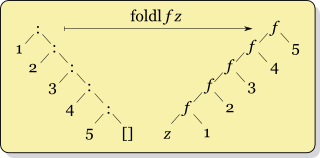
\includegraphics[height=0.30\textheight]{input_src/Left-fold-transformation.png} 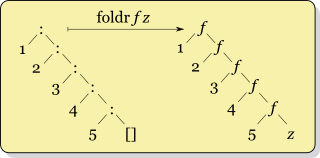
\includegraphics[height=0.30\textheight]{input_src/Right-fold-transformation.png}
	\end{center}
\end{frame}

\begin{frame}[fragile]
	\frametitle{Fold expression}
	\begin{lstlisting}[language=C++]
template<typename... Args>
bool all(Args... args) { return (... && args); }

bool b = all(true, true, true, false);
// ((true && true) && true) && false\end{lstlisting}

	\begin{lstlisting}[language=C++]
template<typename... Args>
long long sum(Args... args) { return (args + ...); }

long long b = sum(1, 2, 3, 4);
// 1 + (2 + (3 + 4))\end{lstlisting}
\end{frame}

\begin{frame}[fragile]
	\frametitle{Fold expression}
	\begin{alertblock}{\textit{left fold} ou \textit{right fold} ?}
		\begin{lstlisting}[language=C++]
template<typename... Args>
double div(Args... args) { return (... / args); }

div(1.0, 2.0, 3.0);      // 0.166667
// (1.0 / 2.0) / 3.0\end{lstlisting}

		\begin{lstlisting}[language=C++]
template<typename... Args>
double div(Args... args) { return (args / ...); }

div(1.0, 2.0, 3.0);      // 1.5
// 1.0 / (2.0 / 3.0)\end{lstlisting}
	\end{alertblock}
\end{frame}

\begin{frame}[fragile]
	\frametitle{Fold expression}
	\begin{itemize}
		\item Si le \textit{parameter pack} est vide, le résultat est
		\begin{itemize}
			\item \lstinline|true| pour l'opérateur \lstinline|&&|
			\item \lstinline|false| pour l'opérateur \lstinline||||
			\item \lstinline|void()| pour l'opérateur \lstinline|,|
		\end{itemize}
	\end{itemize}

	\begin{alertblock}{Attention}
		\begin{itemize}
			\item Un \textit{parameter pack} vide est une erreur pour les autres opérateurs
		\end{itemize}
	\end{alertblock}
\end{frame}

\begin{frame}[fragile]
	\frametitle{Fold expression}
	\begin{itemize}
		\item Compatible avec des opérateurs non arithmétiques ni logiques
	\end{itemize}

	\begin{lstlisting}[language=C++]
template<typename ...Args>
void FoldPrint(Args&&... args) {
  (cout << ... << forward<Args>(args)) << '\n'; }

FoldPrint(10, 'a', "ert"s);\end{lstlisting}

	\begin{itemize}
		\item Y compris \og ,\fg{} qui va donner une séquence d'actions
	\end{itemize}

	\begin{lstlisting}[language=C++]
template<typename T, typename... Args>
void push_back_vec(std::vector<T>& v, Args&&... args) {
  (v.push_back(args), ...); }

vector<int> foo;
push_back_vec(foo, 10, 20, 56);\end{lstlisting}

	\hfill
	\href{https://godbolt.org/#z:OYLghAFBqd5QCxAYwPYBMCmBRdBLAF1QCcAaPECAMzwBtMA7AQwFtMQByARg9KtQYEAysib0QXACx8BBAKoBnTAAUAHpwAMvAFYTStJg1DIApACYAQuYukl9ZATwDKjdAGFUtAK4sGe1wAyeAyYAHI%2BAEaYxCAAbFykAA6oCoRODB7evnrJqY4CQSHhLFEx8baY9vkMQgRMxASZPn4JdpgO6bX1BIVhkdF6CnUNTdmtwz3BfSUDXACUtqhexMjsHOYAzMHI3lgA1CYbbk5DxJish9gmGgCCm9u7mAdHp8HAl9d3ZlsMO177hzcADd2kRiB9bp8vKkjHtmGwFIkmKs9kN0CAQLRCNExApDlZIbcCJgWIkDMTAQQAJ6JRisTAAOiZexuxGAeI2V1uEVQnj2YloEFZ7KZDP5bIUc0%2BJgA7ASbns9mcCMsGHsIKKDmZYuZYuL2VKNvLZQARaVEklkpgUo7U2nwxnM4Ucrk3WgCYB7d2whQ%2BIUSzX1A3SuWfRXK1XqoMKLUWPaiw3GmVmwk3Ymk8mYSk0ulsTXOiE3dBLCL0L34IH%2BkXM6NSyGh27hzAq4hqjXMgD0%2Bsl%2BJDKbuFoz1qztpzDvzEsLxa8paexArVYUgYldbuDYVSubkYg0b2XYTvfr/c%2B6atNrcdtzT1FBc5nyBqDw6D2ADFPOhlMRggRF7rdcvg3reVFQgNEMTQLwCGeNxAXjZlAVgsCQH4YgAHd6nQQFb2wHcVzmaDYLAdYAFY3AYIjDzXY9BzPEcLzHek9gAFVIPZL3HJ1JzvW4HyfPZEmhBAAH0ImRABrISQWQUCCHREApLBQEmI%2BbU9iBViC21f8axXENgPVIEGQEhRhNE5AxNwg1WIPI0%2B3NG5vz2FgmGCCBV1lfSkIgqCEKOVFZIxHlPDERIECYAi/IFCACGILxMFYmK4oS2L4r2KhcUwfDfLcPYKNI8j1ls1NFS8pYfKORC/QSPYzFYjZWMkLKKr8vKyIooqBw3UrIIinLaAXLgGQ0VizCGuqhqamCWo4XKZuypUBrGmqlo2Cbetmkx8va41G1fd9P2/CAuGG2amCI1jzDMaICEunsOrDfy5IUkhAW/S40t5SjFWM0zxMk9pqF5VjjpGk7iNiRMHpQndINQPY8D2EAPtQVdFQ8h6SoClAyvWhH5qIjaOrR5MHu68qppy1qCso01Pg4BZaE4YjeD8DgtFIVBOBgyxrFRJYVieTYeFIAhNHphYxJAYjhsZjhJBZsWOc4XgFBAYbRbZ%2BnSDgWAkEwVR2lhsgKEshRlEMSohAQVBUNZ4W0FJOhrXSc2QloK2bdZ9mHcSOgBmALgzFqn2/eIUJ6WV0gQ/oYgAHlII923Ff19pnUjlPkFqfBWd4fhBBEMR2CkGRBEUFR1E10hdASAwjBQaxrH0PAIlV2AHRAIKhlIEEYm4GVmbmBZUESapVY4ABaNFDhNUwecsLgZT2ceAHUBSX5f9Zi8Lx9pdBDEcZAVf51ZBlk4JXct62k%2B4XgYswNZhdQ4gmESMWGaZhXK85jhsAN5Ajb2KoAAHLEcesRJB7GAMgZAexA4MjMOqbmVhLCsVwIQEgWoNjzFvm/BYCBzhYBiG5Ugktpb6E4PLUgXteDfxVmrEWuDyEcDMJ/dmtCGGa0Ht3aIqRnCSCAA%3D%3D}{
\includegraphics[height=0.5cm]{input_src/play-button.png}}
\end{frame}

\subsection*{Range-based for loop}
\begin{frame}[fragile]
	\frametitle{Contraintes du range-based for loop}
	\begin{itemize}
		\item Utilisation possible de types différents pour \lstinline|end| et \lstinline|begin|
		\item Permet de traiter des paires d'itérateurs
		\item \ldots{} mais aussi un itérateur et une taille
		\item \ldots{} ou un itérateur et une sentinelle de fin
		\item Compatible avec les travaux sur Range TS
	\end{itemize}
\end{frame}

\subsection*{classe}
\begin{frame}[fragile]
	\frametitle{Héritage de constructeur}
	\begin{itemize}
		\item Visibilité des constructeurs hérités avec leurs paramètres par défaut

\note[item]{En C++11, les constructeurs avec paramètres par défaut (ou ellipses) étaient injectés en omettant valeurs par défaut (version avec le paramètre sans valeur par défaut et version sans le paramètre) et ellipse}

		\item Comportement identique aux autres fonctions héritées
	\end{itemize}

\note[item]{Le choix C++11 posait davantage de problèmes (pas de redéfinition avec valeur par défaut possible, multiples constructeurs par copie/déplacement, erreur de SFINAE, etc.)}

	\begin{alertblock}{Attention}
		\begin{itemize}
			\item Casse du code C++11 valide
		\end{itemize}
	\end{alertblock}

	\begin{lstlisting}[language=C++]
struct Foo { Foo(int a, int b = 0); };
struct Bar : Foo {
  Bar(int a); using Foo::Foo; };
struct Baz : Foo {
  Baz(int a, int b = 0); using Foo::Foo; };

Bar bar(0); // Ambigu (OK en C++11)
Baz baz(0); // OK (Ambigu en C++11)\end{lstlisting}

\note[item]{En C++11, \lstinline|Bar| hérite de deux constructeurs - l'un avec deux paramètres \lstinline|int| sans valeur par défaut et l'autre avec un paramètre \lstinline|int| qui est surchargé par le constructeur de \lstinline|Bar|}
\note[item]{En C++11, \lstinline|Baz| hérite de deux constructeurs - l'un avec deux paramètres \lstinline|int| sans valeur par défaut et l'autre avec un paramètre \lstinline|int| - et défini un constructeur avec deux \lstinline|int| dont un avec une valeur par défaut}
\note[item]{En C++17, \lstinline|Bar| hérite d'un constructeur avec deux paramètres \lstinline|int| dont une valeur par défaut et défini un constructeur avec un paramètre \lstinline|int|}
\note[item]{En C++17, \lstinline|Baz|  hérite d'un constructeur avec deux paramètres \lstinline|int| dont un avec une valeur par défaut qu'il redéfini}
\end{frame}

\subsection*{Exception}
\begin{frame}[fragile]
	\frametitle{\lstinline|noexcept|}
	\begin{itemize}
		\item \lstinline|noexcept| fait partie du type des fonctions

		\begin{lstlisting}[language=C++]
void use_func(void (*func)() noexcept);
void my_func();

use_func(&my_func);       // Ne compile plus\end{lstlisting}

\note[item]{Une surcharge sans \lstinline|noexcept| doit être ajoutée}

		\item Les fonctions \lstinline|noexcept| peuvent être convertie en fonctions non \lstinline|noexcept|
	\end{itemize}	
\end{frame}

\begin{frame}[fragile]
	\frametitle{\lstinline|std::uncaught_exceptions()|}
	\begin{itemize}
		\item Retourne le nombre d'exceptions lancées (ou relancées) et non encore attrapées du thread courant
	\end{itemize}

	\begin{lstlisting}[language=C++]
if(uncaught_exceptions()) {
  ... }\end{lstlisting}

	\begin{block}{Motivation}
		\begin{itemize}
			\item Comportement différent d'un destructeur en présence d'exception

\note[item]{P.ex. rollback}
		\end{itemize}
	\end{block}
\end{frame}

\subsection*{Littéraux}
\begin{frame}[fragile]
	\frametitle{Caractères littéraux UTF-8}
	\begin{itemize}
		\item Caractère UTF-8 préfixé par \lstinline|u8|
		\item Erreur si le caractère n'est pas représentable par un unique code point UTF-8
	\end{itemize}

	\begin{lstlisting}[language=C++]
char x = u8'x';\end{lstlisting}

\note[item]{Uniformisation avec les chaînes}
\end{frame}

\subsection*{Template}
\begin{frame}[fragile]
	\frametitle{Déduction de template dans les constructeurs}
	\begin{itemize}
		\item Déduction des paramètres templates d'une classe à la construction
		\item Plus de déclaration explicite des paramètres template
		\item Ni de \textit{make helpers}
	\end{itemize}

\note[item]{Généralisation de la déduction de paramètres template aux constructeurs}
\note[item]{Avant la déduction ne fonctionnait que pour les fonctions membres, pas pour les constructeurs}

	\begin{lstlisting}[language=C++]
pair<int, double> p(2, 4.5);
auto t = make_tuple(4, 3, 2.5);

// Devient

pair p(2, 4.5);
tuple t(4, 3, 2.5);\end{lstlisting}

\note[item]{Fonctionne avec \lstinline|pair p()|, \lstinline|pair p\{\}| et \lstinline|pair()| mais pas, pour l'instant, avec \lstinline|pair\{\}|}
\end{frame}

\begin{frame}[fragile]
	\frametitle{Déduction de template dans les constructeurs}
	\begin{itemize}
		\item Permet de fournir une lambda en paramètre template sans la déclarer
	\end{itemize}

	\begin{lstlisting}[language=C++]
template<class Func> struct Foo { 
  Foo(Func f) : func(f) {} 
  Func func; };

Foo([&](int i) { ... });\end{lstlisting}

	\vskip 10mm plus 10fill
	\hfill
	\href{https://godbolt.org/#g:!((g:!((g:!((h:codeEditor,i:(filename:'1',fontScale:14,fontUsePx:'0',j:1,lang:c%2B%2B,selection:(endColumn:1,endLineNumber:29,positionColumn:1,positionLineNumber:29,selectionStartColumn:1,selectionStartLineNumber:1,startColumn:1,startLineNumber:1),source:'%23include+%3Ciostream%3E%0A%23include+%3Ctuple%3E%0A%23include+%3Cutility%3E%0A%0Atemplate%3Cclass+Func%3E+struct+Foo%0A%7B%0A++Foo(Func+f)+:+func(f)%0A++%7B%0A++%7D%0A%0A++void+operator()+(int+i)%0A++%7B%0A++++func(i)%3B%0A++%7D%0A%0A++Func+func%3B%0A%7D%3B%0A%0Aint+main()%0A%7B%0A++std::pair+p(2,+4.5)%3B%0A++std::tuple+t(4,+3,+2.5)%3B%0A++std::cout+%3C%3C+p.second+%3C%3C+%22+%22+%3C%3C+std::get%3C0%3E(t)+%3C%3C+%22%5Cn%22%3B%0A%0A++int+a+%3D+2%3B%0A++Foo+foo(%5B%26%5D(int+i)+%7Bstd::cout+%3C%3C+a+*+i+%3C%3C+!'%5Cn!'%3B%7D)%3B%0A++foo(5)%3B%0A%7D%0A'),l:'5',n:'0',o:'C%2B%2B+source+%231',t:'0')),k:50,l:'4',n:'0',o:'',s:0,t:'0'),(g:!((h:executor,i:(argsPanelShown:'1',compilationPanelShown:'0',compiler:g122,compilerName:'',compilerOutShown:'0',execArgs:'',execStdin:'',fontScale:14,fontUsePx:'0',j:1,lang:c%2B%2B,libs:!((name:boost,ver:'175')),options:'-std%3Dc%2B%2B17+-Wall+-Wextra+-pedantic',source:1,stdinPanelShown:'1',tree:'1',wrap:'0'),l:'5',n:'0',o:'Executor+x86-64+gcc+12.2+(C%2B%2B,+Editor+%231)',t:'0')),header:(),k:50,l:'4',n:'0',o:'',s:0,t:'0')),l:'2',n:'0',o:'',t:'0')),version:4}{
\includegraphics[height=0.5cm]{input_src/play-button.png}}
\end{frame}

\begin{frame}[fragile]
\frametitle{Déduction de template dans les constructeurs}
	\begin{block}{Note}
		\begin{itemize}
			\item Rend obsolète plusieurs \textit{make helper} (\lstinline|std::make_pair()|, \lstinline|std::make_tuple()|, \ldots)
		\end{itemize}
	\end{block}

	\begin{alertblock}{Attention}
		\begin{itemize}
			\item Ne permet pas la déduction partielle
		\end{itemize}

		\begin{lstlisting}[language=C++]
tuple<int> t(1, 2, 3);  // Erreur\end{lstlisting}
	\end{alertblock}

\note[item]{Il faut donc fournir tous les paramètres templates ou aucun}
\end{frame}

\begin{frame}[fragile]
	\frametitle{\lstinline|template <auto>|}
	\begin{itemize}
		\item Déduction du type des paramètres templates numériques
	\end{itemize}

	\begin{lstlisting}[language=C++]
template <auto value> void foo() {}
foo<10>();  // int\end{lstlisting}

	\begin{lstlisting}[language=C++]
template <typename Type, Type value> 
  constexpr Type FOO = value;
constexpr auto const foo = FOO<int, 100>;

// Devient

template <auto value> constexpr auto FOO = value;
constexpr auto const foo = FOO<100>;\end{lstlisting}

	\vskip 10mm plus 10fill
	\hfill
	\href{https://godbolt.org/#g:!((g:!((g:!((h:codeEditor,i:(filename:'1',fontScale:14,fontUsePx:'0',j:1,lang:c%2B%2B,selection:(endColumn:1,endLineNumber:10,positionColumn:1,positionLineNumber:10,selectionStartColumn:1,selectionStartLineNumber:1,startColumn:1,startLineNumber:1),source:'%23include+%3Ciostream%3E%0A%0Atemplate+%3Cauto+value%3E+constexpr+auto+FOO+%3D+value%3B%0A%0Aint+main()%0A%7B%0A++constexpr+auto+const+foo+%3D+FOO%3C100%3E%3B%0A++std::cout+%3C%3C+foo+%3C%3C+%22%5Cn%22%3B%0A%7D%0A'),l:'5',n:'0',o:'C%2B%2B+source+%231',t:'0')),k:50,l:'4',n:'0',o:'',s:0,t:'0'),(g:!((h:executor,i:(argsPanelShown:'1',compilationPanelShown:'0',compiler:g122,compilerName:'',compilerOutShown:'0',execArgs:'',execStdin:'',fontScale:14,fontUsePx:'0',j:1,lang:c%2B%2B,libs:!((name:boost,ver:'175')),options:'-std%3Dc%2B%2B17+-Wall+-Wextra+-pedantic',source:1,stdinPanelShown:'1',tree:'1',wrap:'0'),l:'5',n:'0',o:'Executor+x86-64+gcc+12.2+(C%2B%2B,+Editor+%231)',t:'0')),header:(),k:50,l:'4',n:'0',o:'',s:0,t:'0')),l:'2',n:'0',o:'',t:'0')),version:4}{
\includegraphics[height=0.5cm]{input_src/play-button.png}}
\end{frame}

\begin{frame}[fragile]
	\frametitle{Template \& contraintes d'utilisation}
	\begin{itemize}
		\item \lstinline|typename| autorisé dans les déclarations de \textit{template template parameters}
	\end{itemize}

	\begin{lstlisting}[language=C++]
template <template <typename> typename C, typename T>
//                            ^^^^^^^^
struct Foo { C<T> data; };

foo<std::vector, int> bar;\end{lstlisting}

\note[item]{Auparavant, il fallait obligatoirement utiliser \lstinline|class|, alors que \lstinline|typename| était valide partout ailleurs}
\end{frame}

\begin{frame}[fragile]
	\frametitle{Template \& contraintes d'utilisation}
	\begin{itemize}
		\item Évaluation constante de tous les arguments templates \og non-types\fg{}
		\item Y compris pointeurs, références, pointeurs sur membres, \ldots
	\end{itemize}

	\begin{lstlisting}[language=C++]
template<int* P> struct Foo { 
  int operator()() { return *P; } };
int N = 5;

Foo<&N> foo;     // OK
foo();           // 5

constexpr int* bar() { return &N; }
Foo<bar()> foo2; // OK
foo2();          // 5\end{lstlisting}
\end{frame}

\subsection*{Programmation fonctionnelle}
\begin{frame}[fragile]
	\frametitle{Capture de \lstinline|*this|}
	\begin{itemize}
		\item Capture \lstinline|*this| par valeur

\note[item]{Jusqu'à présent, on ne pouvait pas capturer la classe courante, seulement des attributs de celle-ci}
	\end{itemize}

	\begin{lstlisting}[language=C++]
[*this]() { ... }
[=, *this]() { ... }\end{lstlisting}

	\begin{lstlisting}[language=C++]
struct Foo {
  auto bar() {
    return [*this] { cout << s << endl; }; }
  std::string s; };

auto baz = Foo{"baz"}.bar();
baz();     // Affiche baz\end{lstlisting}
\end{frame}

\begin{frame}[fragile]
	\frametitle{Lambdas et expressions constantes}
	\begin{itemize}
		\item Lambdas autorisées dans les expressions constantes
		\item Si l'initialisation de chaque capture est possible dans l'expression constante
	\end{itemize}

	\begin{lstlisting}[language=C++]
constexpr int AddEleven(int n)
  { return [n] { return n+11; }(); }

AddEleven(5);   // 16\end{lstlisting}
\end{frame}

\begin{frame}[fragile]
	\frametitle{Lambdas et expressions constantes}
	\begin{itemize}
		\item Déclaration \lstinline|constexpr| de lambda possible 
		\item Explicitement via \lstinline|constexpr|
	\end{itemize}

	\begin{lstlisting}[language=C++]
auto ID = [] (int n) constexpr { return n; };
constexpr int I = ID(3);\end{lstlisting}

	\begin{itemize}
		\item Implicitement \lstinline|constexpr| lorsque les exigences sont satisfaites
	\end{itemize}

\note[item]{Les lambdas sont donc \lstinline|constexpr| par défaut}

	\begin{lstlisting}[language=C++]
auto ID = [] (int n) { return n; };
constexpr int I = ID(3);\end{lstlisting}
\end{frame}

\begin{frame}[fragile]
	\frametitle{Lambdas et expressions constantes}
	\begin{itemize}
		\item Fermeture de type littéral si les données sont des littéraux
	\end{itemize}

	\begin{lstlisting}[language=C++]
constexpr auto add = [] (int n, int m) {
  auto L = [=] { return n; };
  auto R = [=] { return m; };
  return [=] { return L() + R(); }; };

add(3, 4)()   // 7\end{lstlisting}

	\vskip 10mm plus 10fill
	\hfill
	\href{https://godbolt.org/#z:OYLghAFBqd5QCxAYwPYBMCmBRdBLAF1QCcAaPECAMzwBtMA7AQwFtMQByARg9KtQYEAysib0QXACx8BBAKoBnTAAUAHpwAMvAFYTStJg1DIApACYAQuYukl9ZATwDKjdAGFUtAK4sGe1wAyeAyYAHI%2BAEaYxCAAzABspAAOqAqETgwe3r56KWmOAkEh4SxRMQm2mPYFDEIETMQEWT5%2BXJXVGXUNBEVhkdF6CvWNzTltQ929JWUSAJS2qF7EyOwc5rHByN5YANQmsW5OQ8SYrPvYJhoAgpdXaAxDmKpJxDvBBDtX6OjY9ABujAg7x2DFmtxMAHYrNcdjsTgQlgw9gBWCwMEzIgAieyhcMwCOISKR1h2XC4%2BwsOMxEDBsWhNwhmPB12BLCYwRp4Kht1hkPpsNhQ3QIBQiw%2B%2BzcEs%2B31%2BmABDAgyNmewOUrAa2RbgY6opPKpzKuvO5MIFTC8RB2AElsfsbaiMdigYIQcr7o9nq8%2BXiCUSKfq6XrYW6CE8Xm9nZaVdjrRBYrT%2BQKhSK0OaVZKDla02qNVqdQGTZCmdc9XzAzszRbrVGUVYsTsnR9QTjKfDESC/YXdSagwJ3WHgZHbVbqXGu4bEwRhaLUxKpYPVRmdZrtWt8%2BPO8WC8bxz2HiGPeXzahy99qxja47gQxSOGPiwwd2BU/ny/X6XH6/P1/YRXjwEz/asRMnWXqtoS7Z0v6CbfjBr6/jsABKAFWEBDrNt6bYsB2jJjrBeHPmBxKAcBNq4oROwBDSeyWIhnKQZ2a74fhDHQTsSbTuKC5uCe6CxjekizFRs6LjmK64fqxY4dcHDzLQnDIrwfgcFopCoJwkqWCSCiLMsmDUbEPCkAQmgyfMADWIDIho%2BicJIikmapnC8AoIDWcZykyaQcCwEgTyYMgR5kBQEANMACjKIYVRCAgqAAO5KYZaAsEkdBMDUEUhLQ0VxUpKlJSl9AxMAXBmGYpD5XQ0ShKwqy8BVhUAPLmtl8UOX5yBXMQYVOaQ7V1PgSm8PwggiGI7BSDIgiKCo6geaQuhtAYRgoNY1j6HgEQubAzBsCAESoKkBCkACMTcBCCmzPMqBJDULkcAAtEKtqmJplhcBCOz3QA6mItCfV9TwEMQTCfUkmDoIYjjIM5OkrIMk7BBlUUxa13C8EDmCrIZsXA0kJmyfJ9lzWpHDYKo/mBTsqgABzxPd8SSDswDIMgpJmAAdGY9YaVYlg3rghAkPpXCzOj%2BPzAgpxYDENKkBZVk2RwdmkLlvAk85rlGeLitmETKnq1rHmXcd0RpM4khAA%3D%3D}{
\includegraphics[height=0.5cm]{input_src/play-button.png}}
\end{frame}

\begin{frame}[fragile]
	\frametitle{\lstinline|std::invoke()|}
	\begin{itemize}
		\item Appelle l'appelable fourni en paramètre
		\item \ldots{} en fournissant la liste de paramètres
		\item \ldots{} et en retournant le retour de l'appelable
	\end{itemize}

	\begin{lstlisting}[language=C++]
int foo(int i) {
  return i + 42; }

invoke(&foo, 8);  // 50\end{lstlisting}
\end{frame}

\begin{frame}[fragile]
	\frametitle{\lstinline|std::invoke()|}
	\begin{itemize}
		\item Fonctionne également avec des fonctions membres
		\item \ldots{} le premier paramètre fourni est l'objet à utiliser
	\end{itemize}

	\begin{lstlisting}[language=C++]
struct Foo {
  int bar(int i) {
    return i + 42; } };

Foo foo;
invoke(&Foo::bar, foo, 8);  // 50\end{lstlisting}

	\begin{block}{Motivation}
		\begin{itemize}
			\item Syntaxe unique d'appel d'appelable
		\end{itemize}
	\end{block}

	\vskip 10mm plus 10fill
	\hfill
	\href{https://godbolt.org/#g:!((g:!((g:!((h:codeEditor,i:(filename:'1',fontScale:14,fontUsePx:'0',j:1,lang:c%2B%2B,selection:(endColumn:1,endLineNumber:24,positionColumn:1,positionLineNumber:24,selectionStartColumn:1,selectionStartLineNumber:1,startColumn:1,startLineNumber:1),source:'%23include+%3Ciostream%3E%0A%23include+%3Cfunctional%3E%0A%0Astatic+int+foo(int+i)%0A%7B%0A++return+i+%2B+42%3B%0A%7D%0A%0Astruct+Bar%0A%7B%0A++int+baz(int+i)%0A++%7B%0A++++return+i+%2B+42%3B%0A++%7D%0A%7D%3B%0A%0Aint+main()%0A%7B%0A++std::cout+%3C%3C+std::invoke(%26foo,+8)+%3C%3C+!'%5Cn!'%3B%0A%0A++Bar+bar%3B%0A++std::cout+%3C%3C+std::invoke(%26Bar::baz,+bar,+8)+%3C%3C+!'%5Cn!'%3B%0A%7D%0A'),l:'5',n:'0',o:'C%2B%2B+source+%231',t:'0')),k:50,l:'4',n:'0',o:'',s:0,t:'0'),(g:!((h:executor,i:(argsPanelShown:'1',compilationPanelShown:'0',compiler:g122,compilerName:'',compilerOutShown:'0',execArgs:'',execStdin:'',fontScale:14,fontUsePx:'0',j:1,lang:c%2B%2B,libs:!((name:boost,ver:'175')),options:'-std%3Dc%2B%2B17+-Wall+-Wextra+-pedantic',source:1,stdinPanelShown:'1',tree:'1',wrap:'0'),l:'5',n:'0',o:'Executor+x86-64+gcc+12.2+(C%2B%2B,+Editor+%231)',t:'0')),header:(),k:50,l:'4',n:'0',o:'',s:0,t:'0')),l:'2',n:'0',o:'',t:'0')),version:4}{
\includegraphics[height=0.5cm]{input_src/play-button.png}}
\end{frame}

\begin{frame}[fragile]
	\frametitle{\lstinline|std::not_fn()|}
	\begin{itemize}
		\item Construction de \textit{function object} en niant un appelable
	\end{itemize}

	\begin{lstlisting}[language=C++]
bool LessThan10(int a) {
  return a < 10; }
	
vector foo = { 1, 6, 3, 8, 14, 42, 2 };
count_if(begin(foo), end(foo), not_fn(LessThan10)); // 2\end{lstlisting}

	\begin{block}{Dépréciation}
		\begin{itemize}
			\item Dépréciation de \lstinline|std::not1| et \lstinline|std::not2|
		\end{itemize}
	\end{block}
\end{frame}

\subsection*{Type traits}
\begin{frame}[fragile]
	\frametitle{Alias de traits}
	\begin{itemize}
		\item Ajout du suffixe \lstinline|_v| aux traits de la forme \lstinline|is_...|
		\item Suppression de \lstinline|::value|
	\end{itemize}

	\begin{lstlisting}[language=C++]
template <typename T>
enable_if_t<is_integral<T>::value, T>
sqrt(T t);

// Devient 

template <typename T>
enable_if_t<is_integral_v<T>, T>
sqrt(T t);\end{lstlisting}
\end{frame}

\begin{frame}[fragile]
	\frametitle{Nouveaux traits}
	\begin{itemize}
		\item Nouveaux traits
		\begin{itemize}
			\item \lstinline|is_swappable_with|, \lstinline|is_swappable|, \lstinline|is_nothrow_swappable_with| et \lstinline|is_nothrow_swappable| : objets échangeables
			\item \lstinline|is_callable| et \lstinline|is_nothrow_callable| : objet appelable
			\item \lstinline|void_t| conversion en \lstinline|void|

\note[item]{Surtout utile en méta-programmation via \lstinline|enable_if| et le SFINAE}

		\end{itemize}
		\item Méta-fonctions sur les traits
		\begin{itemize}
			\item \lstinline|std::conjunction| : et logique entre traits
			\item \lstinline|std::disjunction| : ou logique entre traits
			\item \lstinline|std::negation| : négation d'un trait
		\end{itemize}
	\end{itemize}

	\begin{lstlisting}[language=C++]
// foo disponible si tous ls Ts... ont le meme type
template<typename T, typename... Ts>
enable_if_t<conjunction_v<is_same<T, Ts>...>>
foo(T, Ts...) {}\end{lstlisting}
\end{frame}

\subsection*{Attributs}
\begin{frame}[fragile]
	\frametitle{Gestion des attributs}
	\begin{itemize}
		\item Usage étendu aux déclarations de \lstinline|namespace|
	\end{itemize}

	\begin{lstlisting}[language=C++]
namespace [[ Attribut ]] foo {}\end{lstlisting}

	\begin{itemize}
		\item Et aux valeurs d'une énumération
	\end{itemize}

	\begin{lstlisting}[language=C++]
enum foo {
  FOO_1 [[ Attribut ]],
  FOO_2 };\end{lstlisting}
\end{frame}

\begin{frame}[fragile]
	\frametitle{Gestion des attributs}
	\begin{itemize}
		\item Attributs inconnus doivent être ignorés

\note[item]{Clarification de la norme, auparavant un compilateur pouvait lever une erreur car rien n'était précisé.}
\note[item]{Maintenant, il ne le peut plus et doit seulement ignorer l'attribut (éventuellement avec un avertissement).}

		\item \lstinline|using| des attributs non standard
	\end{itemize}

	\begin{lstlisting}[language=C++]
[[ nsp::kernel, nsp::target(cpu,gpu) ]]
foo();

// Devient

[[ using nsp: kernel, target(cpu,gpu) ]]
foo();\end{lstlisting}
\end{frame}

\begin{frame}[fragile]
	\frametitle{Attribut \lstinline|[[ fallthrough ]]|}
	\begin{itemize}
		\item Dans un \lstinline|switch| avant un \lstinline|case| ou \lstinline|default|
		\item Indique qu'un cas se poursuit intentionnellement dans le cas suivant
		\item Incitation à ne pas lever d'avertissement dans ce cas
	\end{itemize}

	\begin{lstlisting}[language=C++]
switch(foo) {
  case 1:
  case 2:
    ...
[[ fallthrough ]];
  case 3:   // Idealement : pas de warning
    ...
  case 4:   // Idealement : warning
    ...
    break; }\end{lstlisting}

\note[item]{Les compilateurs offraient déjà des mécanismes similaires (\lstinline|__attribute__ ((fallthrough));| ou \lstinline|[[gnu::fallthrough]]| sur GCC, voire des commentaires à un format précis)}
\note[item]{Généralement pas d'avertissement sur des case vides (cas 1-2 ici)}

	\vskip 10mm plus 10fill
	\hfill
	\href{https://godbolt.org/#g:!((g:!((g:!((h:codeEditor,i:(filename:'1',fontScale:14,fontUsePx:'0',j:1,lang:c%2B%2B,selection:(endColumn:12,endLineNumber:19,positionColumn:12,positionLineNumber:19,selectionStartColumn:12,selectionStartLineNumber:19,startColumn:12,startLineNumber:19),source:'%23include+%3Ciostream%3E%0A%0Aint+main()%0A%7B%0A++int+foo+%3D+1%3B%0A%0A++switch(foo)%0A++%7B%0A++++case+1:%0A++++case+2:%0A++++++std::cout+%3C%3C+%22Cas+1-2%5Cn%22%3B%0A%23if+1%0A++++++%5B%5B+fallthrough+%5D%5D%3B%0A%23endif%0A%0A++++case+3:%0A++++++std::cout+%3C%3C+%22Cas+3%5Cn%22%3B%0A%0A++++case+4:%0A++++++std::cout+%3C%3C+%22Cas+4%5Cn%22%3B%0A++++++break%3B%0A%0A++++default:%0A++++++std::cout+%3C%3C+%22Cas+default%5Cn%22%3B%0A++++++break%3B%0A++%7D%0A%7D%0A'),l:'5',n:'0',o:'C%2B%2B+source+%231',t:'0')),k:50,l:'4',n:'0',o:'',s:0,t:'0'),(g:!((h:executor,i:(argsPanelShown:'1',compilationPanelShown:'0',compiler:g122,compilerName:'',compilerOutShown:'0',execArgs:'',execStdin:'',fontScale:14,fontUsePx:'0',j:1,lang:c%2B%2B,libs:!((name:boost,ver:'175')),options:'-std%3Dc%2B%2B17+-Wall+-Wextra+-pedantic',source:1,stdinPanelShown:'1',tree:'1',wrap:'0'),l:'5',n:'0',o:'Executor+x86-64+gcc+12.2+(C%2B%2B,+Editor+%231)',t:'0')),header:(),k:50,l:'4',n:'0',o:'',s:0,t:'0')),l:'2',n:'0',o:'',t:'0')),version:4}{
\includegraphics[height=0.5cm]{input_src/play-button.png}}
\end{frame}

\begin{frame}[fragile]
	\frametitle{Attribut \lstinline|[[ nodiscard ]]|}
	\begin{itemize}
		\item Indique que le retour d'une fonction ne devrait pas être ignorée
	\end{itemize}

	\begin{lstlisting}[language=C++]
[[ nodiscard ]] int foo() { return 5; }

foo();  // Idealement : warning\end{lstlisting}

	\begin{itemize}
		\item Incitation à lever un avertissement dans le cas contraire
	\end{itemize}

	\begin{block}{Note}
		\begin{itemize}
			\item Conversion implicite en \lstinline|void| pour supprimer l'avertissement
		\end{itemize}
		\begin{lstlisting}[language=C++]
(void)foo();\end{lstlisting}

\note[item]{Au moins avec GCC, à voir avec Visual C++ et Clang} 
	\end{block}
\end{frame}

\begin{frame}[fragile]
	\frametitle{Attribut \lstinline|[[ nodiscard ]]|}
	\begin{itemize}
		\item Possible sur la déclaration d'un type (classe, structure ou énumération)
		\item Indique qu'un retour de ce type ne devrait jamais être ignoré
	\end{itemize}

	\begin{lstlisting}[language=C++]
struct [[ nodiscard ]] Bar {};
Bar baz() { return Bar{}; }

baz();  // Idealement : warning\end{lstlisting}

	\vskip 10mm plus 10fill
	\hfill
	\href{https://godbolt.org/#g:!((g:!((g:!((h:codeEditor,i:(filename:'1',fontScale:14,fontUsePx:'0',j:1,lang:c%2B%2B,selection:(endColumn:1,endLineNumber:22,positionColumn:1,positionLineNumber:22,selectionStartColumn:1,selectionStartLineNumber:1,startColumn:1,startLineNumber:1),source:'%23include+%3Ciostream%3E%0A%0A%5B%5B+nodiscard+%5D%5D+static+int+foo()%0A%7B%0A++return+5%3B%0A%7D%0A%0Astruct+%5B%5B+nodiscard+%5D%5D+Bar%0A%7B%0A%7D%3B%0A%0Astatic+Bar+baz()%0A%7B%0A++return+Bar%7B%7D%3B%0A%7D%0A%0Aint+main()%0A%7B%0A++foo()%3B%0A++baz()%3B%0A%7D%0A'),l:'5',n:'0',o:'C%2B%2B+source+%231',t:'0')),k:50,l:'4',n:'0',o:'',s:0,t:'0'),(g:!((h:executor,i:(argsPanelShown:'1',compilationPanelShown:'0',compiler:g122,compilerName:'',compilerOutShown:'0',execArgs:'',execStdin:'',fontScale:14,fontUsePx:'0',j:1,lang:c%2B%2B,libs:!((name:boost,ver:'175')),options:'-std%3Dc%2B%2B17+-Wall+-Wextra+-pedantic',source:1,stdinPanelShown:'1',tree:'1',wrap:'0'),l:'5',n:'0',o:'Executor+x86-64+gcc+12.2+(C%2B%2B,+Editor+%231)',t:'0')),header:(),k:50,l:'4',n:'0',o:'',s:0,t:'0')),l:'2',n:'0',o:'',t:'0')),version:4}{
\includegraphics[height=0.5cm]{input_src/play-button.png}}
\end{frame}

\begin{frame}[fragile]
	\frametitle{Attribut \lstinline|[[ maybe_unused ]]|}
	\begin{itemize}
		\item Sur une classe, structure, fonction, variable, paramètre, \ldots
		\item Indique qu'un élément peut ne pas être utilisé
		\item Incitation à ne pas lever d'avertissement en cas de non-utilisation
	\end{itemize}

	\begin{lstlisting}[language=C++]
[[ maybe_unused ]]
int foo([[ maybe_unused ]] int a,
        [[ maybe_unused ]] long b) {}\end{lstlisting}

	\begin{itemize}
		\item Ne devrait pas lever d'avertissement en cas d'utilisation
	\end{itemize}

	\begin{block}{Avant C++17}
		\begin{itemize}
			\item Ne pas nommer les paramètres non utilisés
		\end{itemize}
	\end{block}

	\vskip 10mm plus 10fill
	\hfill
	\href{https://godbolt.org/#g:!((g:!((g:!((h:codeEditor,i:(filename:'1',fontScale:14,fontUsePx:'0',j:1,lang:c%2B%2B,selection:(endColumn:1,endLineNumber:17,positionColumn:1,positionLineNumber:17,selectionStartColumn:1,selectionStartLineNumber:1,startColumn:1,startLineNumber:1),source:'%23include+%3Ciostream%3E%0A%0A%23if+0%0A%5B%5B+maybe_unused+%5D%5D+static+int+foo(%5B%5B+maybe_unused+%5D%5Dint+a,%0A++++++++++++++++++++++++++++++++++%5B%5B+maybe_unused+%5D%5D+int+b)%0A%23else%0Astatic+int+foo(int+a,%0A+++++++++++++++int+b)%0A%23endif%0A%7B%0A++return+0%3B%0A%7D%0A%0Aint+main()%0A%7B%0A%7D%0A'),l:'5',n:'0',o:'C%2B%2B+source+%231',t:'0')),k:50,l:'4',n:'0',o:'',s:0,t:'0'),(g:!((h:executor,i:(argsPanelShown:'1',compilationPanelShown:'0',compiler:g112,compilerName:'',compilerOutShown:'0',execArgs:'',execStdin:'',fontScale:14,fontUsePx:'0',j:1,lang:c%2B%2B,libs:!((name:boost,ver:'175')),options:'-std%3Dc%2B%2B17+-Wall+-Wextra+-pedantic',source:1,stdinPanelShown:'1',tree:'1',wrap:'0'),l:'5',n:'0',o:'Executor+x86-64+gcc+11.2+(C%2B%2B,+Editor+%231)',t:'0')),header:(),k:50,l:'4',n:'0',o:'',s:0,t:'0')),l:'2',n:'0',o:'',t:'0')),version:4}{
\includegraphics[height=0.5cm]{input_src/play-button.png}}
\end{frame}

\begin{frame}[fragile]
	\frametitle{Attributs C++17 - Conclusion}
	\begin{exampleblock}{Do}
		\begin{itemize}
			\item Utilisez les attributs pour indiquer vos intentions
		\end{itemize}

\note[item]{Au delà de l'information pour le compilateur et d'autres outils, c'est aussi une documentation à l'intention des lecteurs et correcteurs}
	\end{exampleblock}

	\begin{block}{Au delà du compilateur}
		\begin{itemize}
			\item Prise en compte par d'autres outils souhaitable

\note[item]{Autres outils : générateurs de documentation, analyseurs statique de code}
		\end{itemize}
	\end{block}
\end{frame}

\subsection*{Multi-threading}
\begin{frame}[fragile]
	\frametitle{\lstinline|std::shared_mutex|}
	\begin{itemize}
		\item Similaire à \lstinline|std::mutex| avec deux niveaux d'accès
		\begin{itemize}
			\item Exclusif : possible si le verrou n'est pas pris
			\item Partagé : possible si le verrou n'est pas pris en exclusif
		\end{itemize}
		\item API identique à \lstinline|std::mutex| pour l'accès exclusif
		\item API similaire pour l'accès partagé
		\begin{itemize}
			\item \lstinline|lock_shared|
			\item \lstinline|try_lock_shared|
			\item \lstinline|unlock_shared|
		\end{itemize}
	\end{itemize}

	\begin{block}{Note}
		\begin{itemize}
			\item Équivalent \textit{non-timed} de \lstinline|std::shared_timed_mutex|
		\end{itemize}
	\end{block}
\end{frame}

\begin{frame}[fragile]
	\frametitle{\lstinline|std::scoped_lock|}
	\begin{itemize}
		\item Acquisition de plusieurs mutex
	\end{itemize}

	\begin{lstlisting}[language=C++]
mutex first_mutex;
mutex second_mutex;

scoped_lock lck(first_mutex, second_mutex);\end{lstlisting}
\end{frame}

\subsection*{Library fundamentals TS}
\begin{frame}[fragile]
	\frametitle{\lstinline|std::apply()|}
	\begin{itemize}
		\item Appel de fonction depuis un \textit{tuple-like} d'argument
	\end{itemize}

	\begin{lstlisting}[language=C++]
void foo(int a, long b, string c) {}

tuple bar{42, 5L, "bar"s};
apply(foo, bar);\end{lstlisting}

	\begin{itemize}
		\item Fonctionne sur tout ce qui supporte \lstinline|std::get()| et \lstinline|std::tuple_size|
		\item Notamment \lstinline|std::pair| et \lstinline|std::array|
	\end{itemize}

	\begin{lstlisting}[language=C++]
array<int, 3> baz{1, 54, 3};
apply(foo, baz);\end{lstlisting}

	\begin{itemize}
		\item \lstinline|std::make_from_tuple()| permet de construire un objet depuis un \textit{tuple-like}
	\end{itemize}

	\vskip 10mm plus 10fill
	\hfill
	\href{https://godbolt.org/#g:!((g:!((g:!((h:codeEditor,i:(filename:'1',fontScale:14,fontUsePx:'0',j:1,lang:c%2B%2B,selection:(endColumn:37,endLineNumber:13,positionColumn:37,positionLineNumber:13,selectionStartColumn:37,selectionStartLineNumber:13,startColumn:37,startLineNumber:13),source:'%23include+%3Ciostream%3E%0A%23include+%3Ctuple%3E%0A%23include+%3Carray%3E%0A%23include+%3Cstring%3E%0A%0Ausing+namespace+std::literals%3B%0A%0Astatic+void+foo(int+a,+long+b,+std::string+c)%0A%7B%0A++std::cout+%3C%3C+a+%3C%3C+!'+!'+%3C%3C+b+%3C%3C+!'+!'+%3C%3C+c+%3C%3C+!'%5Cn!'%3B%0A%7D%0A%0Astatic+void+bar(int+a,+int+b,+int+c)%0A%7B%0A++std::cout+%3C%3C+a+%3C%3C+!'+!'+%3C%3C+b+%3C%3C+!'+!'+%3C%3C+c+%3C%3C+!'%5Cn!'%3B%0A%7D%0A%0Aint+main()%0A%7B%0A++%7B%0A++++std::tuple+baz%7B42,+5L,+%22bar%22s%7D%3B%0A++++std::apply(foo,+baz)%3B%0A++%7D%0A%0A++%7B%0A++++std::array%3Cint,+3%3E+baz%7B42,+5,+12%7D%3B%0A++++std::apply(bar,+baz)%3B%0A++%7D%0A%7D%0A'),l:'5',n:'0',o:'C%2B%2B+source+%231',t:'0')),k:50,l:'4',n:'0',o:'',s:0,t:'0'),(g:!((h:executor,i:(argsPanelShown:'1',compilationPanelShown:'0',compiler:g122,compilerName:'',compilerOutShown:'0',execArgs:'',execStdin:'',fontScale:14,fontUsePx:'0',j:1,lang:c%2B%2B,libs:!((name:boost,ver:'175')),options:'-std%3Dc%2B%2B17+-Wall+-Wextra+-pedantic',source:1,stdinPanelShown:'1',tree:'1',wrap:'0'),l:'5',n:'0',o:'Executor+x86-64+gcc+12.2+(C%2B%2B,+Editor+%231)',t:'0')),header:(),k:50,l:'4',n:'0',o:'',s:0,t:'0')),l:'2',n:'0',o:'',t:'0')),version:4}{
\includegraphics[height=0.5cm]{input_src/play-button.png}}
\end{frame}

\begin{frame}[fragile]
	\frametitle{\lstinline|std::optional|}
	\begin{itemize}
		\item Gestion d'objet dont la présence est optionnelle
	\end{itemize}

	\begin{alertblock}{Restriction}
		\begin{itemize}
			\item Ne peut pas contenir des références, des tableaux C, \lstinline|void| ni être vide
		\end{itemize}
	\end{alertblock}

	\begin{itemize}
		\item Interface similaire à un pointeur
		\begin{itemize}
			\item Testable via \lstinline|operator bool()|
			\item Accès à l'objet via \lstinline|operator*|
			\item Accès à un membre via \lstinline|operator->|
		\end{itemize}
	\end{itemize}

	\begin{alertblock}{Attention}
		\begin{itemize}
			\item \lstinline|operator*| ou \lstinline|operator->| indéfini sur un \lstinline|std::optional| vide
		\end{itemize}
	\end{alertblock}

	\begin{itemize}
		\item [] \begin{itemize}
			\item \lstinline|std::nullopt| indique l'absence de l'objet
		\end{itemize}
		\item \lstinline|value()| retourne la valeur ou lève l'exception \lstinline|std::bad_optional_access|
		\item \lstinline|value_or()| retourne la valeur ou une valeur par défaut
	\end{itemize}
\end{frame}

\begin{frame}[fragile]
	\frametitle{\lstinline|std::optional|}
	\begin{itemize}
		\item Supporte la déduction de type
	\end{itemize}

	\begin{lstlisting}[language=C++]
optional foo(10);	// std::optional<int>\end{lstlisting}

	\begin{itemize}
		\item Supporte la construction en-place
	\end{itemize}

	\begin{lstlisting}[language=C++]
optional<complex<double>> foo{in_place, 3.0, 4.0};\end{lstlisting}

	\begin{itemize}
		\item Y compris depuis un \lstinline|std::initializer_list|
	\end{itemize}

	\begin{lstlisting}[language=C++]
optional<vector<int>> foo(in_place, {1, 2, 3});\end{lstlisting}

	\begin{itemize}
		\item Existence du \textit{helper} \lstinline|std::make_optional|
	\end{itemize}

	\begin{lstlisting}[language=C++]
auto foo = make_optional(3.0);
auto bar = make_optional<complex<double>>(3.0, 4.0);\end{lstlisting}
\end{frame}

\begin{frame}[fragile]
	\frametitle{\lstinline|std::optional|}
	\begin{itemize}
		\item Changement de la valeur via \lstinline|reset()|, \lstinline|swap()|, \lstinline|emplace()| ou \lstinline|operator=|
		\item Comparaison naturelle des valeurs contenues 
	\end{itemize}

	\begin{lstlisting}[language=C++]
optional<int> deux(2), dix(10);

dix > deux;   // true	
dix < deux;   // false
dix == 10;    // true\end{lstlisting}

	\begin{itemize}
		\item En prenant en compte \lstinline|std::nullopt|
	\end{itemize}

	\begin{lstlisting}[language=C++]
optional<int> none, dix(10);

dix > none;       // true	
dix < none;       // false
none == 10;       // false
none == nullopt;  // true\end{lstlisting}

\note[item]{\lstinline|std::nullopt| est inférieur à toutes valeurs}
\end{frame}

\begin{frame}[fragile]
	\frametitle{\lstinline|std::optional|}
	\begin{alertblock}{\lstinline|std::optional<bool>| ? \lstinline|std::optional<T*>| ?}
		\begin{itemize}
			\item Utilisez des booléens \og trois états\fg{} (Boost.tribool)
			\item Utilisez des pointeurs bruts
		\end{itemize}
	\end{alertblock}

	\begin{exampleblock}{Do}
		\begin{itemize}
			\item Préférez \lstinline|optional| aux pointeurs bruts pour gérer des données optionnelles
		\end{itemize}

\note[item]{Sémantique plus précise, pas de risque de tentative de libération ou de fuite mémoire, \lstinline|value()| et \lstinline|value_or()| permettent de simplifier l'usage}
	\end{exampleblock}

	\begin{block}{En attendant C++17}
		\begin{itemize}
			\item Utilisez Boost.Optional
		\end{itemize}
	\end{block}

	\vskip 10mm plus 10fill
	\hfill
	\href{https://godbolt.org/#z:OYLghAFBqd5QCxAYwPYBMCmBRdBLAF1QCcAaPECAMzwBtMA7AQwFtMQByARg9KtQYEAysib0QXACx8BBAKoBnTAAUAHpwAMvAFYTStJg1DIApACYAQuYukl9ZATwDKjdAGFUtAK4sGe1wAyeAyYAHI%2BAEaYxCAAHNIADqgKhE4MHt6%2BekkpjgJBIeEsUTHxtpj2eQxCBEzEBBk%2BflzllWk1dQQFYZHRegq19Y1ZLQOd3UUlEgCUtqhexMjsHOYAzMHI3lgA1Carbk4DxJise9gmGgCCaxtbmLv7qAlVYmcX12brDJteO3tuXkctEIAE83lcbt87g83GgWAl6KpwR8vj8/vsAG6YBwkZHvMaOZDbAboEAgJ4vWj/YIEM7bfioCA07ZMabvEwAdisV222zwVAgTAe2G2GjZPN522OBAWDBZe25l15FSU70lUswMuIcpJZIYXlotApCvZHIAIuyrsyWExghBxdcuWrdk6JbzdeTnmlXvsPXCEZgkft0PMIvQ3qsRRE6pyLB7ggB9BFMJakbarAB0GjTkiznItq0V6r98wIMP%2B2wAVNHiOX9tswCsAKxuBiNk0Qt0swGobbRgBeDzNxIIpJANoA1pgExTvVTfaOyf7Ef8Q14w5gI9gIE2s2mAGxZtmF53uxcoUt1txVgdXhvN1vtk8S/OWpUuouSj2zgQ%2BtwerEcWIalBC3Ps6ggeMGCTAxUw/FptjMNNVnzY9P15fhiAgNAGAGbsiD5MsQBvOoHXVM8xzQQE70IO9G3vDt3wopdL3%2BCt2xbNsVmfd9X07XjXSYkcxx/ZhaHA2s9mHBkIEkMw0NPPkBRrMjyJLai2Pras6joh8uMY9UVU3LtmIvDT9grcwzAxPAsBMTirMYxTvy9X9xNvKT6VQRkAFp5IMyV%2BQgAdVOLc8qLLTTr20wcooYzin3Q7YjMU0yIrvKybLshyzDMAK%2BOuF9BLCkTXLEiShy83z/J49UCGIMEu1jVLhJY8y3ArGsMwxMQvEwe1dPsx9uKSgr1VEAhkAQbCBDwj1o3QGcyrEBMUyWBQFHMfdktCj8WvUyKLPrTAMwAdwQJgCAGuKOOGgLeTGl0LX4h7iq/c9RLECrPJkvyFK7A67y6nrvGnEhZPkwaEpG50Ctht7TM%2B%2BcDlAyNtiwLxVAgGqkpcykQNpNH8CxrgxScgHwtYo7r3m7yDFoBILvu1qzMOjr6wgYnhXRzBMemKG7ufABOAB6EXtnqvrnMp9qK05vBVBhHm%2BYF/ThbF%2BkxFVCnKKp9nr3lxWpM80n%2BZuvTEouIXeQ1yXjIE57CoE3GPuW5GaTpBgBE3Wr3tK/H9g9omFYgU3yaEwG4tpzwxEZphmcj6ntkN7mvZCM2k9utXuWt8j1Vt4gpZ1tq2blrmKzTzAM/1%2BLBZzvP8/FqgtftkqS7vCBK6HE2xVVy2NFzhvtg15vaG1iOZdLjmu%2BN1Zhw9fVDQpav2ItmGB4LouHdNR2OFmWhOCbXg/A4LRSFQTgOssaxiXmRZ7jWHhSAITQ99mCcQCbbMD44SRj9f8%2BnBeAKBANmF%2Bp896kDgLAJAgZsQ9jIBQQUxBgAKGUIYCoQgECoFOifJ%2B/o6CXTSOgkItAsE4JPmfAh9AYjAC4LlUg1DoihFYMsXgTDiAAHlATkNwQAuByBLgoJARwXgAiaj4BPrwfgggRBiHYFIGQghFAqHUBA0gugWgGCMCgaw1h9B4AiCA2AzA2AgAiN5AYpAsQxG4ByI%2B0xZiiRET5EkUlTDX0sFwDk2wfIAHUxDiX8YGeqQofIJEwOgQwhJgF3yWP0UcwQSGYOwXw7gvB6qYGWE/U6xAmAJFfvvQ%2B/91EXw4NgVQ8CiC1lULEfcPl9ySG2MAZARJ6EZjMMnK%2BVhLBplwIQEguxPhcGmBkwpswEAnCwDEe0pAP5f30JwP%2BpBKG8DKcA0Bz9xmLI4GYEpZ91lbIgY46x0QUjOEkEAA%3D%3D}{
\includegraphics[height=0.5cm]{input_src/play-button.png}}
\end{frame}

\begin{frame}[fragile]
	\frametitle{\lstinline|std::any|}
	\begin{itemize}
		\item \lstinline|void*| \textit{type-safe} contenant un objet de n'importe quel type (ou vide)
		\item Implémentation de \textit{Type-erasure}

\note[item]{Pour les données, tout comme \lstinline|std::function| est un \textit{type-erasure} pour les appelables}

		\item Type contenu dépend de la valeur assignée
	\end{itemize}

	\begin{lstlisting}[language=C++]
any a = 1;  // int
a = 3.14;   // double
a = true;   // bool\end{lstlisting}
\end{frame}

\begin{frame}[fragile]
	\frametitle{\lstinline|std::any|}
	\begin{itemize}
		\item Supporte la construction en-place
	\end{itemize}

	\begin{lstlisting}[language=C++]
any a(in_place_type<complex<double>>, 3.0, 4.0);\end{lstlisting}

	\begin{itemize}
		\item \textit{Helper} \lstinline|std::make_any|
	\end{itemize}

	\begin{lstlisting}[language=C++]
any a = make_any<complex<double>>(3.0, 4.0);\end{lstlisting}

	\begin{itemize}
		\item Changement de valeur, éventuellement de type, via l'affectation
	\end{itemize}

	\begin{lstlisting}[language=C++]
std::any a = 1;
a = 3.14;\end{lstlisting}

	\begin{itemize}
		\item \ldots{} ou \lstinline|emplace()|
	\end{itemize}

	\begin{lstlisting}[language=C++]
a.emplace<std::complex<double>>(3.0, 4.0);\end{lstlisting}
\end{frame}

\begin{frame}[fragile]
	\frametitle{\lstinline|std::any|}
	\begin{itemize}
		\item \lstinline|any_cast<Type>()| récupère la valeur
		\item \ldots{} et lève une exception si le type demandé n'est pas correct
	\end{itemize}

	\begin{lstlisting}[language=C++]
any a = 1;
any_cast<int>(a);  // 1
any_cast<bool>(a); // Lance bad_any_cast\end{lstlisting}

	\begin{itemize}
		\item ou récupère l'adresse
		\item \ldots{} et retourne \lstinline|nullptr| si le type demandé n'est pas correct
	\end{itemize}

	\begin{lstlisting}[language=C++]
any a = 1;
int* foo = any_cast<int>(&a);
int* foo = any_cast<bool>(&a);     // nullptr\end{lstlisting}
\end{frame}

\begin{frame}[fragile]
	\frametitle{\lstinline|std::any|}
	\begin{itemize}
		\item \lstinline|reset()| vide le contenu
		\item \lstinline|has_value()| teste la vacuité
		\item \lstinline|type()| récupère l'information du type courant

\note[item]{L'information de type récupérée ainsi est \textit{implementation-dependant} et non utilisable tel quel mais peut être comparé au retour de \lstinline|type_id|}
	\end{itemize}

	\begin{block}{En attendant C++17 \ldots}
		\begin{itemize}
			\item Utilisez Boost.Any
		\end{itemize}
	\end{block}

	\vskip 10mm plus 10fill
	\hfill
	\href{https://godbolt.org/#z:OYLghAFBqd5QCxAYwPYBMCmBRdBLAF1QCcAaPECAMzwBtMA7AQwFtMQByARg9KtQYEAysib0QXACx8BBAKoBnTAAUAHpwAMvAFYTStJg1DIApACYAQuYukl9ZATwDKjdAGFUtAK4sGIAGykrgAyeAyYAHI%2BAEaYxBIAHKQADqgKhE4MHt6%2BASlpGQKh4VEssfFcSXaYDplCBEzEBNk%2BfoHVtQL1jQTFkTFxibYNTS257SO9Yf1lg5UAlLaoXsTI7BzmAMxhyN5YANQmm25OCgTEmKxH2CYaAIJbO3uYh8eGAJ7Xtw9m2wy7XgORzcXkctEIn02N3uj3%2Bz1ebjQLGS9FUXxh9zCBH2LCYYQg82%2BJgA7FZ7vtDqTvhSKWd0CAQB99kxXgARfZcI5ku40/Z0hloUEI4F8gj0xkMd4AfVEZ2BWOuECY82Fx32YA2AFY3AwNVyieSaSyjuzNgA6KT6w20sUC5bY4Ei/kS6WygjA9DLaL0RXK1VudVanV6zbc6lGtn7c5eTBWnk052Ch3HJ22kDRVCeMTJBDGlNq50fGVMOXHDOeX0qx1qvXa3UbUMGn7bKj7DThm3ipP%2B0Xiotu%2BWCSs92vBhth36uPBUJu8phmzDIgxrYGJ1BLzBo46erze2NQxXmjSkfaSM0aQmN629u1C6sBwuS4ultxrjdbtw7vdfKFKqv5gNR3rOMKRJVlZ0pbleUfd5mUjTkr3jTtb2TNxUz7J8B2OBVf3Mfw/XvQ4zDMfYAFoiJIwiACoYOfd1sKHXCzHw/80JrINgMQ6C027QjaKwz8vR9JiWJHDiQygylwIxeMSUk5CXWZCBnTCKUUSYNYpQId5kn3V8ePXFFNw9IT9xuKETyPE8zwvECEwMu8AJvF06NXAz3xM3dhPM7A/zEkw6wk8MwIguSO2cpk83ZZ1cQAa0wKUPjcrtDNRTzvwPX8rNPc9L3k5zeKc/iS3o/SUo87dTJ/XyCKcoCgsNEKZNAqlrxg5k7IUwq2IfNNywMWgczzHrmTNXMFClAA3MQYwJfzAvHcKov2TVOoK%2B0e2dfrs1zHt53GqaZswOb7w1QM9rNbTdIJM1mDYE66vExbGuJaSHle74OEWWhOE1Xg/A4LRSFQTg0Msaw%2BWWVYXi2HhSAITQvsWWKQE1Y8fo4SR/sR4HOF4BQQGPBHAa%2B0g4FgJBNxqUESHIShGmABRlEMTBaCEBBUAAdwBuGkWSOgmEcARmfCNmOe5nG%2BboQZgC4YjSCl%2BhiAiVh1l4RW4gAeVBdmuYBoGqeQO5iEZvGglUGp6nwAHeH4QQRDEdgpBkQRFBUdQSdIXQuH0QxjGsax9DwaICdgO72HLM5SEmwZuGJP75kWVBkiFhgCY4Ui6RNUxwcsLhiTIgB1MRaCLzdzhZUjdPQQxHGQfGobWPQ6TCEXWd1iXuF4c5MHWOHOeIJhkkR77fuxz2QY4bALeQGniH2VQEn8Uj/EkfZgGQZAOTMM0SIgMGrEsE9cEIEgiM2Lh5m7kfFgQS4sHiAlSBRtH9E4LHSH13hJ/xwn4Zvt%2BHAzDjyBj/f%2BJNE7RziOkZwkggA%3D%3D%3D}{
\includegraphics[height=0.5cm]{input_src/play-button.png}}
\end{frame}

\begin{frame}[fragile]
	\frametitle{\lstinline|std::string_view|}
	\begin{itemize}
		\item Vue sur une séquence contiguë de caractères
		\item Quatre spécialisations standard (une par type de caractères)
		\item Référence non possédante sur une séquence pré-existante
		\item Pas de modification de la séquence depuis la vue
		\item Constructible depuis \lstinline|std::string|, une chaîne C ou un pointeur et une taille
	\end{itemize}

	\begin{alertblock}{Attention !}
		\begin{itemize}
			\item Pas de \lstinline|\0| terminal systématique
			\item La chaîne référencée doit vivre au moins aussi longtemps que la vue
		\end{itemize}
	\end{alertblock}
\end{frame}

\begin{frame}[fragile]
	\frametitle{\lstinline|std::string_view|}
	\begin{itemize}
		\item Accès aux caractères : \lstinline|operator[]|, \lstinline|at()|, \lstinline|front()|, \lstinline|back()|, \lstinline|data()|
		\item Modification des bornes : \lstinline|remove_prefix()| et \lstinline|remove_suffix()|
		\item Accès à la taille et à la taille maximale : \lstinline|size()|, \lstinline|length()| et \lstinline|max_size()|
		\item Test de vacuité : \lstinline|empty()|
		\item Construction d'une chaîne depuis la vue : \lstinline|to_string()|
		\item Copie d'une partie de la vue : \lstinline|copy()|
		\item Construction d'une vue sur une sous-partie de la vue : \lstinline|substr()|
		\item Comparaison avec une autre vue ou une chaîne : \lstinline|compare()|
		\item Recherche : \lstinline|find()|, \lstinline|rfind()|, \lstinline|find_first_of()|, \lstinline|find_last_of()|, \lstinline|find_first_not_of()|, \lstinline|find_last_not_of|
		\item Comparaison lexicographique : \lstinline|==|, \lstinline|!=|, \lstinline|<=|, \lstinline|>=|, \lstinline|<| et \lstinline|>|
		\item Affichage : \lstinline|operator<<|
	\end{itemize}
\end{frame}

\begin{frame}[fragile]
	\frametitle{\lstinline|std::string_view|}
	\begin{lstlisting}[language=C++]
string foo = "Lorem ipsum dolor sit amet";

string_view bar(&foo[0], 11);
cout << bar.size() << " - " << bar << '\n';
// 11 - Lorem ipsum

bar.remove_suffix(6);
cout << bar.size() << " - " << bar << '\n';
// 5 - Lorem\end{lstlisting}

	\begin{exampleblock}{Performances}
		\begin{itemize}
			\item Souvent meilleures que les fonctionnalités équivalentes de \lstinline|string|
			\item Mais pas toujours, donc mesurez
		\end{itemize} 

\note[item]{Et que boost.split}
\note[item]{Notamment car il y a moins d'allocation mémoire}
\note[item]{La contrepartie c'est qu'il n'y a pas de chaîne de construite ni de modification possible}
\note[item]{Travailler à base de chaîne peut être plus rapide lorsque le compilateur peut optimiser correctement le code avec les chaîne, si on construit une chaîne au final p.ex.}
	\end{exampleblock}

	\vskip 6mm plus 10fill
	\hfill
	\href{https://godbolt.org/#z:OYLghAFBqd5QCxAYwPYBMCmBRdBLAF1QCcAaPECAMzwBtMA7AQwFtMQByARg9KtQYEAysib0QXACx8BBAKoBnTAAUAHpwAMvAFYTStJg1DIApACYAQuYukl9ZATwDKjdAGFUtAK4sGe1wAyeAyYAHI%2BAEaYxCBmAOykAA6oCoRODB7evnrJqY4CQSHhLFEx8baY9vkMQgRMxASZPn5cFVXptfUEhWGR0XoKdQ1N2a2DXT3FpRIAlLaoXsTI7BzmAMzByN5YANQma25Og8SYrPvYJhoAguub25h7B8fBwOeXN2YbDFteu/tuzyMAH0AG54TAAdze13ewQIOxYTGCEBm7xMcSs1x2ewx72x2MG6BAIEBwB2/FQjwAInszGYAiRMCwdnhEgofDt0J4SDs8jtWJgCKQdmgGEoHILFvz8Ik8ApkC8dpVCAA6HZCTDoHYMAQ7YhyrwKFXmMz7TE3LH4wnE0mg8EQnYReoQcwANgpJgArBYNF6qcKuFxUWtzfjeQQiSgFvD/v9HfUVakAF6YFGPNxxk07AC0tLM6bjTuIBYOOzAq09bgY5bNaMt2I93t9npp%2Bxp5doNZDeKtEeJaC8MYOhYTydTMxLbjzOensdLRcnZYrVa7od7kYHQ4z8/qXp9fsXNcr1dW3Zh9fjxBVJxYqBBmCB7KoNFUEFdwbXBL7UcHi6LibwFM0znKcs1zLMQMvQ9lxPWtLXRKk6yubF0U/EUEHqclUFQPc1gPNscQscsiN4JcmHLYVy2IGs4kQs9kPXG0CH1YEwUhS9qGw4Ux1QKgsNQD8ey/Ddoz/UdAPHRcwNnYcd2LSCjxXU81wQtFaPeDg5loThPV4PwOC0UhUE4DNLGsXkFiWB51h4UgCE0TS5gAaxAT0NH0ThJD0hyjM4XgFBAdz7IMzTSDgWAkEwVRMGQQcSHISh6mABRlEMSohAQVAIX02y0BYWUDGqVKQloDKsv0wy8oK/pgC4OlSCquholCAU/Ia1B8qa4gAHlBzK7KfKimKrmIZK2qG5BanwfTeH4QQRDEdgpBkQRFBUdQQtIXRWgMIwUGsax9DwCIAtgZg2BACJsMGUh7xibg4l0mY5lQRJqgCjhs0JNtTDMywuDiHMAHUxFoYGouYpgc0STVDEcZB/Ms5YBgjYJivSzKBu4XhmMwFZbIhYgmESBytJ07zNuMjhsGi2KiGLVQAA5XWzV1JB2YBkGQHY6pVfMIFMqxLGFXBCB5GyZhx0m5gQU4sBiFFSBctyPI4LzSAq3gqf8wK7Ol1WzApwztb1kLntu6JUmcSQgA%3D%3D%3D}{
\includegraphics[height=0.5cm]{input_src/play-button.png}}
\end{frame}

\begin{frame}[fragile]
	\frametitle{Mémoire}
	\begin{itemize}
		\item \lstinline|std::shared_ptr| et \lstinline|std::weak_ptr| sur des tableaux
	\end{itemize}

	\begin{lstlisting}[language=C++]
std::shared_ptr<int[]> foo(new int[10]);\end{lstlisting}

	\begin{alertblock}{Pas de \lstinline|std::make_shared()|}
		\begin{itemize}
			\item \lstinline|std::make_shared()| ne supporte pas les tableaux en C++17
		\end{itemize}
	\end{alertblock}

	\begin{itemize}
		\item Évolutions des allocateurs

\note[item]{\textit{Type-erased allocator}, \textit{polymorphic allocator}, \textit{memory ressources}}
\note[item]{Gestion de l'alignement des \textit{Over-Aligned Data}}

		\item Classe de gestion de pools de ressources (synchronisés ou non)
	\end{itemize}

	\begin{block}{Note}
		\begin{itemize}
			\item Pointeur intelligent sans responsabilité dans le TS \lstinline|observer_ptr|
			\item Mais pas dans le périmètre accepté pour C++17
		\end{itemize}
	\end{block}
\end{frame}

\begin{frame}[fragile]
	\frametitle{Algorithmes}
	\begin{itemize}
		\item Recherche d'une séquence dans une autre
		\begin{itemize}
			\item Trois foncteurs de recherche : \textit{default}, Boyer-Moore et Boyer-Moore-Horspoll
			\item \lstinline|std::search()| encapsule l'appel à un des foncteurs
		\end{itemize}
		\item Échantillonnage
		\begin{itemize}
			\item \lstinline|std::sample()| extrait aléatoirement n éléments d'un ensemble
		\end{itemize}
	\end{itemize}

	\begin{lstlisting}[language=C++]
string in = "abcdefgh", out;
sample(begin(in), end(in), back_inserter(out), 
       5, mt19937{random_device{}()});\end{lstlisting}

	\vskip 10mm plus 10fill
	\hfill
	\href{https://godbolt.org/#g:!((g:!((g:!((h:codeEditor,i:(filename:'1',fontScale:14,fontUsePx:'0',j:1,lang:c%2B%2B,selection:(endColumn:1,endLineNumber:20,positionColumn:1,positionLineNumber:20,selectionStartColumn:1,selectionStartLineNumber:1,startColumn:1,startLineNumber:1),source:'%23include+%3Ciostream%3E%0A%23include+%3Cstring%3E%0A%23include+%3Calgorithm%3E%0A%23include+%3Crandom%3E%0A%23include+%3Cctime%3E%0A%0Aint+main()%0A%7B%0A++std::string+in+%3D+%22abcdefgh%22%3B%0A++std::string+out%3B%0A++std::mt19937+gen%7Bstatic_cast%3Cunsigned+long%3E(time(nullptr))%7D%3B%0A++std::sample(std::begin(in),+std::end(in),+std::back_inserter(out),+5,+gen)%3B%0A%0A++for(auto+it+:+out)%0A++%7B%0A++++std::cout+%3C%3C+it+%3C%3C+!'+!'%3B%0A++%7D%0A++std::cout+%3C%3C+!'%5Cn!'%3B%0A%7D%0A'),l:'5',n:'0',o:'C%2B%2B+source+%231',t:'0')),k:50,l:'4',n:'0',o:'',s:0,t:'0'),(g:!((h:executor,i:(argsPanelShown:'1',compilationPanelShown:'0',compiler:g122,compilerName:'',compilerOutShown:'0',execArgs:'',execStdin:'',fontScale:14,fontUsePx:'0',j:1,lang:c%2B%2B,libs:!((name:boost,ver:'175')),options:'-std%3Dc%2B%2B17+-Wall+-Wextra+-pedantic',source:1,stdinPanelShown:'1',tree:'1',wrap:'0'),l:'5',n:'0',o:'Executor+x86-64+gcc+12.2+(C%2B%2B,+Editor+%231)',t:'0')),header:(),k:50,l:'4',n:'0',o:'',s:0,t:'0')),l:'2',n:'0',o:'',t:'0')),version:4}{
\includegraphics[height=0.5cm]{input_src/play-button.png}}
\end{frame}

\begin{frame}[fragile]
	\frametitle{PGCD et PPCM}
	\begin{itemize}
		\item Ajout des fonctions \lstinline|gcd| et \lstinline|lcm|
		\item Initialement prévu pour des versions ultérieures
		\item \ldots{} mais suffisamment simples et élémentaires pour C++17 
	\end{itemize}

	\begin{lstlisting}[language=C++]
gcd(12, 18);   // 6
lcm(12, 18);   // 36\end{lstlisting}

	\vskip 10mm plus 10fill
	\hfill
	\href{https://godbolt.org/#g:!((g:!((g:!((h:codeEditor,i:(filename:'1',fontScale:14,fontUsePx:'0',j:1,lang:c%2B%2B,selection:(endColumn:1,endLineNumber:9,positionColumn:1,positionLineNumber:9,selectionStartColumn:1,selectionStartLineNumber:1,startColumn:1,startLineNumber:1),source:'%23include+%3Ciostream%3E%0A%23include+%3Cnumeric%3E%0A%0Aint+main()%0A%7B%0A++std::cout+%3C%3C+std::gcd(12,+18)+%3C%3C+!'%5Cn!'%3B%0A++std::cout+%3C%3C+std::lcm(12,+18)+%3C%3C+!'%5Cn!'%3B%0A%7D%0A'),l:'5',n:'0',o:'C%2B%2B+source+%231',t:'0')),k:50,l:'4',n:'0',o:'',s:0,t:'0'),(g:!((h:executor,i:(argsPanelShown:'1',compilationPanelShown:'0',compiler:g122,compilerName:'',compilerOutShown:'0',execArgs:'',execStdin:'',fontScale:14,fontUsePx:'0',j:1,lang:c%2B%2B,libs:!((name:boost,ver:'175')),options:'-std%3Dc%2B%2B17+-Wall+-Wextra+-pedantic',source:1,stdinPanelShown:'1',tree:'1',wrap:'0'),l:'5',n:'0',o:'Executor+x86-64+gcc+12.2+(C%2B%2B,+Editor+%231)',t:'0')),header:(),k:50,l:'4',n:'0',o:'',s:0,t:'0')),l:'2',n:'0',o:'',t:'0')),version:4}{
\includegraphics[height=0.5cm]{input_src/play-button.png}}
\end{frame}

\subsection*{Filesystem TS}
\begin{frame}[fragile]
	\frametitle{Filesystem TS}
	\begin{itemize}
		\item Gestion des systèmes de fichiers
		\item Adapté à l'OS et au système de fichiers utilisés
		\item Manipulation des chemins et noms de fichiers
	\end{itemize}

	\begin{lstlisting}[language=C++]
path foo("/home/foo");
path bar(foo / "bar.txt");
bar.filename();    // bar.txt
bar.extension();   // .txt
bar.native();      // std::string
bar.c_str();       // const char*\end{lstlisting}
\end{frame}

\begin{frame}[fragile]
	\frametitle{Filesystem TS}
	\begin{itemize}
		\item Manipulation des répertoires, des fichiers et de leurs méta-datas
		\begin{itemize}
			\item Copie : \lstinline|copy_file()|, \lstinline|copy()|
			\item Création de répertoires : \lstinline|create_directory()|, \lstinline|create_directories()|

\note[item]{Différence : création du répertoire final seulement ou de tous les répertoires intermédiaires nécessaires}

			\item Création des liens : \lstinline|create_symlink()|, \lstinline|create_hard_link()|
			\item Test d'existence : \lstinline|exists()|
			\item Taille : \lstinline|file_size()|
			\item Type : \lstinline|is_regular_file()|, \lstinline|is_directory()|, \lstinline|is_symlink()|, \lstinline|is_fifo()|, \lstinline|is_socket()|, \ldots
			\item Permissions : \lstinline|permissions()|
			\item Date de dernière écriture : \lstinline|last_write_time()|
			\item Suppression : \lstinline|remove()|, \lstinline|remove_all()|

\note[item]{Différence \lstinline|remove| et \lstinline|remove_all| : suppression récursive pour le second}

			\item Changement de nom : \lstinline|rename()|
			\item Changement de taille : \lstinline|resize_file()|
			\item Chemin du répertoire temporaire : \lstinline|temp_directory_path()|
			\item Chemin du répertoire courant : \lstinline|current_path()|
		\end{itemize}
	\end{itemize}
\end{frame}

\begin{frame}[fragile]
	\frametitle{Filesystem TS}
	\begin{itemize}
		\item Parcours de répertoires
		\begin{itemize}
			\item Entrée du répertoire : \lstinline|directory_entry|
			\item Itérateurs pour le parcours
			\begin{itemize}
				\item Parcours simple : \lstinline|directory_iterator|
				\item Parcours récursif : \lstinline|recursive_directory_iterator|
			\end{itemize}
			\item Construction de l'itérateur de début depuis le chemin du répertoire
			\item Construction de l'itérateur de fin par défaut
		\end{itemize}
		\item \lstinline|std::fstream| constructible depuis \lstinline|path|
	\end{itemize}

	\begin{exampleblock}{Do}
		\begin{itemize}
			\item Utilisez \textit{Filesystem} plutôt que les API C ou systèmes
		\end{itemize}
	\end{exampleblock}

	\begin{block}{En attendant C++17}
		\begin{itemize}
			\item Utilisez Boost.Filesystem
		\end{itemize}
	\end{block}
\end{frame}

\subsection*{Parallelism TS}
\begin{frame}[fragile]
	\frametitle{Parallelism TS}
	\begin{itemize}
		\item Surcharges \og parallèles\fg{} de nombreux algorithmes standard
		\item Politiques d'exécution (séquentielle, parallèle et parallèle+vectorisée)
	\end{itemize}

	\begin{lstlisting}[language=C++]
void bar(int i);

vector<int> foo {0, 5, 42, 58};
for_each(execution::par, begin(foo), end(foo), bar);\end{lstlisting}

	\begin{alertblock}{Attention}
		\begin{itemize}
			\item Pas de gestion intrinsèque des accès concurrents
		\end{itemize}
	\end{alertblock}
\end{frame}

\begin{frame}[fragile]
	\frametitle{Parallelism TS}
	\begin{itemize}
		\item \lstinline|std::for_each_n()| : variante de \lstinline|std::for_each()| prenant l'itérateur de début et une taille et non une paire d'itérateurs

\note[item]{En soi, ce n'est pas lié au parallélisme mais cet algorithme apparait avec ce TS}

		\item \lstinline|std::reduce()| \og ajoute\fg{} tous les éléments de l'ensemble
	\end{itemize}

	\begin{block}{\lstinline|std::reduce()| ou \lstinline|std::accumulate()| ?}
		\begin{itemize}
			\item Ordre des \og additions\fg{} non spécifié dans le cas de \lstinline|std::reduce()|
		\end{itemize}

\note[item]{Le résultat n'est donc pas déterministe dans le cas d'opérations non associatives ou non commutatives (car \lstinline|std::reduce()| regroupe et réarrange les opérations)}
\note[item]{Mais rend cet algorithme parallélisable contrairement à \lstinline|std::accumulate()|}
	\end{block}
\end{frame}

\begin{frame}[fragile]
	\frametitle{Parallelism TS}
	\begin{itemize}
		\item \lstinline|std::exclusive_scan()| construit un ensemble où chaque élément est égal à la somme des éléments de rang strictement inférieur de l'ensemble initial et d'une valeur initiale
	\end{itemize}

	\begin{lstlisting}[language=C++]
vector<int> foo {5, 42, 58}, bar;

exclusive_scan(begin(foo), end(foo), 
               back_inserter(bar), 8);
// bar : 8 13 55\end{lstlisting}
\end{frame}

\begin{frame}[fragile]
	\frametitle{Parallelism TS}
	\begin{itemize}
		\item \lstinline|std::inclusive_scan()| construit un ensemble où chaque élément est égal à la somme des éléments de rang inférieur ou égal de l'ensemble initial et d'une valeur initiale (si présente)
	\end{itemize}

	\begin{lstlisting}[language=C++]
vector<int> foo {5, 42, 58};
vector<int> bar;

inclusive_scan(begin(foo), end(foo), 
               back_inserter(bar), 8);
// bar : 13 55 113\end{lstlisting}

\note[item]{\lstinline|exclusive_scan| et \lstinline|inclusive_scan| sont proche de \lstinline|partial_sum| mais sans garanti d'ordre des \og additions\fg{} avec résultat indéterminé en cas d'opérations non associatives (idem \lstinline|reduce()| / \lstinline|accumulate()|)}
\end{frame}

\begin{frame}[fragile]
	\frametitle{Parallelism TS}
	\begin{itemize}
		\item \lstinline|std::transform_reduce()| : \lstinline|std::reduce()| sur des éléments préalablement transformés
		\item \lstinline|std::transform_exclusive_scan()| : \lstinline|std::exclusive_scan()| sur des éléments préalablement transformés
		\item \lstinline|std::transform_inclusive_scan()| : \lstinline|std::inclusive_scan()| sur des éléments préalablement transformés
	\end{itemize}

	\begin{block}{Note}
		\begin{itemize}
			\item Transformation non appliquée à la graine
		\end{itemize}
	\end{block}

	\vskip 10mm plus 10fill
	\hfill
	\href{https://godbolt.org/#g:!((g:!((g:!((h:codeEditor,i:(filename:'1',fontScale:14,fontUsePx:'0',j:1,lang:c%2B%2B,selection:(endColumn:2,endLineNumber:18,positionColumn:2,positionLineNumber:18,selectionStartColumn:1,selectionStartLineNumber:1,startColumn:1,startLineNumber:1),source:'%23include+%3Ciostream%3E%0A%23include+%3Cvector%3E%0A%23include+%3Cnumeric%3E%0A%0Aint+main()%0A%7B%0A++std::vector%3Cint%3E+foo+%7B5,+42,+58%7D%3B%0A++std::vector%3Cint%3E+bar%3B%0A%0A++std::exclusive_scan(std::begin(foo),+std::end(foo),+std::back_inserter(bar),+8)%3B%0A%0A++for+(const+auto+it+:+bar)%0A++%7B%0A%09++std::cout+%3C%3C+it+%3C%3C+%22+%22%3B%0A++%7D%0A++std::cout+%3C%3C+%22%5Cn%22%3B%0A%7D%0A+'),l:'5',n:'0',o:'C%2B%2B+source+%231',t:'0')),k:50,l:'4',n:'0',o:'',s:0,t:'0'),(g:!((h:executor,i:(argsPanelShown:'1',compilationPanelShown:'0',compiler:g122,compilerName:'',compilerOutShown:'0',execArgs:'',execStdin:'',fontScale:14,fontUsePx:'0',j:1,lang:c%2B%2B,libs:!((name:boost,ver:'175')),options:'-std%3Dc%2B%2B17+-Wall+-Wextra+-pedantic',source:1,stdinPanelShown:'1',tree:'1',wrap:'0'),l:'5',n:'0',o:'Executor+x86-64+gcc+12.2+(C%2B%2B,+Editor+%231)',t:'0')),header:(),k:50,l:'4',n:'0',o:'',s:0,t:'0')),l:'2',n:'0',o:'',t:'0')),version:4}{
\includegraphics[height=0.5cm]{input_src/play-button.png}}
\end{frame}

\subsection*{Mathematical Special Functions}
\begin{frame}[fragile]
	\frametitle{Mathematical Special Functions}
	\begin{itemize}
		\item Une longue histoire datant du TR1
		\item Ajout de fonctions mathématiques particulières
		\begin{itemize}
			\item Fonctions cylindriques de Bessel
			\item Fonctions de Neumann
			\item Polynômes de Legendre
			\item Polynômes de Hermite
			\item Polynômes de Laguerre
			\item \ldots
		\end{itemize}
	\end{itemize}
\end{frame}
\end{document}